%  Manuscript for MDPI Agronomy, Special Issue "Advancing Plant Phenotyping for Precision Crop Growth
%  Monitoring and Forecast Leveraging In Situ, Remote and Proximal Sensing, and AI".
%  Build: cd paper && latexmk -pdf main.tex   (or `make paper` from the project root).
%  All result numbers are macros from numbers.tex, generated by paper/R/export_numbers.R (`make numbers`).

%=================================================================
\documentclass[agronomy,article,submit,pdftex]{Definitions/mdpi}

%=================================================================
% MDPI internal commands - do not modify
\firstpage{1}
\makeatletter
\setcounter{page}{\@firstpage}
\makeatother
\pubvolume{1}
\issuenum{1}
\articlenumber{0}
\pubyear{2026}
\copyrightyear{2026}
\datereceived{ }
\daterevised{ }
\dateaccepted{ }
\datepublished{ }
\hreflink{https://doi.org/}

%=================================================================
% Packages and helper macros
\usepackage{xspace}
\xspaceaddexceptions{\%}   % no space between a number macro and a following percent sign

% Placeholders for facts that only the author can supply and for numbers that have no source yet
\newcommand{\TODO}[1]{\textcolor{red}{[TODO: #1]}}
\newcommand{\NumMissing}[1]{\textcolor{red}{[NUM: #1]}}

% The MDPI class sets a header taller than fancyhdr's default; raise the head height and keep the text block where it is
\AtBeginDocument{\setlength{\headheight}{24.2pt}\addtolength{\topmargin}{-12.2pt}}

% Every result number and design constant (generated; do not edit numbers.tex)
% AUTO-GENERATED by paper/R/export_numbers.R via `make numbers`. Do not edit.
\newcommand{\NumCfgCycleYears}{10\xspace}
\newcommand{\NumCfgMeanYield}{800\xspace}
\newcommand{\NumCfgSigmaA}{150\xspace}
\newcommand{\NumCfgHtwoYield}{0.30\xspace}
\newcommand{\NumCfgHorizon}{25\xspace}
\newcommand{\NumGainTargetPct}{0.5\xspace}
\newcommand{\NumGainScale}{0.13\xspace}
\newcommand{\NumDGtradPerYearCal}{4.0\xspace}
\newcommand{\NumNcellsOK}{5,760\xspace}
\newcommand{\NumNrepsPerCell}{100\xspace}
\newcommand{\NumNcellsNegDiff}{345\xspace}
\newcommand{\NumDGtradPerCycle}{301\xspace}
\newcommand{\NumDGtradPerYear}{30.1\xspace}
\newcommand{\NumDGdiffPerCycle}{8.0\xspace}
\newcommand{\NumDGdiffPct}{2.7\xspace}
\newcommand{\NumDGvsBaseTradPerCycle}{647\xspace}
\newcommand{\NumDGdiffSE}{2.5\xspace}
\newcommand{\NumDGdiffErrZero}{2.4\xspace}
\newcommand{\NumDGdiffErrTen}{4.5\xspace}
\newcommand{\NumDGdiffErrTwenty}{6.7\xspace}
\newcommand{\NumDGdiffErrThirty}{9.2\xspace}
\newcommand{\NumDGdiffErrForty}{11.4\xspace}
\newcommand{\NumDGdiffErrFifty}{13.9\xspace}
\newcommand{\NumNlookupRows}{3,600,000\xspace}
\newcommand{\NumPrNPVpos}{98.4\xspace}
\newcommand{\NumBasePrice}{0.50\xspace}
\newcommand{\NumBaseDisc}{8\xspace}
\newcommand{\NumBaseAdopt}{30\xspace}
\newcommand{\NumBaseArea}{5\xspace}
\newcommand{\NumEAAcycZero}{0.01\xspace}
\newcommand{\NumNPVcycZero}{0.6\xspace}
\newcommand{\NumPrPosCycZero}{93.7\xspace}
\newcommand{\NumEAAcycOne}{0.13\xspace}
\newcommand{\NumNPVcycOne}{6.7\xspace}
\newcommand{\NumPrPosCycOne}{100.0\xspace}
\newcommand{\NumEAAcycTwo}{0.25\xspace}
\newcommand{\NumNPVcycTwo}{13.4\xspace}
\newcommand{\NumPrPosCycTwo}{100.0\xspace}
\newcommand{\NumEAAcycThree}{0.39\xspace}
\newcommand{\NumNPVcycThree}{20.9\xspace}
\newcommand{\NumPrPosCycThree}{100.0\xspace}
\newcommand{\NumEAAperYearCompressed}{0.13\xspace}
\newcommand{\NumStressMedianNPV}{0.8\xspace}
\newcommand{\NumStressMinMarginalNPV}{0.010\xspace}
\newcommand{\NumConsEAAmean}{0.012\xspace}
\newcommand{\NumConsEAAsd}{0.008\xspace}
\newcommand{\NumSobolSoneCyc}{0.29\xspace}
\newcommand{\NumSobolSTCyc}{0.53\xspace}
\newcommand{\NumSobolSoneDisc}{0.16\xspace}
\newcommand{\NumSobolSTDisc}{0.35\xspace}
\newcommand{\NumSobolSonePrice}{0.14\xspace}
\newcommand{\NumSobolSTPrice}{0.32\xspace}
\newcommand{\NumSobolSoneAdopt}{0.07\xspace}
\newcommand{\NumSobolSTAdopt}{0.17\xspace}
\newcommand{\NumSobolSoneErrRed}{0.001\xspace}
\newcommand{\NumSobolSTErrRed}{0.003\xspace}
\newcommand{\NumSobolSoneCostRed}{$<$0.001\xspace}
\newcommand{\NumSobolSTCostRed}{0.001\xspace}
\newcommand{\NumSobolSoneBudget}{$<$0.001\xspace}
\newcommand{\NumSobolSTBudget}{0.001\xspace}
\newcommand{\NumSobolSoneFixCost}{$<$0.001\xspace}
\newcommand{\NumSobolSTFixCost}{0.001\xspace}
\newcommand{\NumSobolSumSone}{0.67\xspace}
\newcommand{\NumSobolSumST}{1.38\xspace}
\newcommand{\NumSobolEconST}{0.84\xspace}
\newcommand{\NumSobolMinorSTmax}{0.003\xspace}
\newcommand{\NumSobolMinorSTsum}{0.006\xspace}
\newcommand{\NumSobolBootMaxShift}{0.001\xspace}
\newcommand{\NumBootB}{120\xspace}
\newcommand{\NumNexactGrid}{720,000\xspace}
\newcommand{\NumSobolCycZeroSTDisc}{0.43\xspace}
\newcommand{\NumSobolCycZeroSTErrRed}{0.35\xspace}
\newcommand{\NumSobolCycZeroSTPrice}{0.31\xspace}
\newcommand{\NumSobolCycZeroSTBudget}{0.20\xspace}
\newcommand{\NumSobolCycZeroSTAdopt}{0.17\xspace}
\newcommand{\NumSobolCycZeroSTCostRed}{0.15\xspace}
\newcommand{\NumSobolCycZeroSTFixCost}{0.10\xspace}
\newcommand{\NumShapleyCyc}{0.43\xspace}
\newcommand{\NumShapleyDisc}{0.21\xspace}
\newcommand{\NumShapleyPrice}{0.21\xspace}
\newcommand{\NumShapleyAdopt}{0.12\xspace}
\newcommand{\NumShapleyErrRed}{0.02\xspace}
\newcommand{\NumShapleyBudget}{0.004\xspace}
\newcommand{\NumShapleyCostRed}{$<$0.001\xspace}
\newcommand{\NumShapleyFixCost}{$<$0.001\xspace}
\newcommand{\NumPawnCyc}{0.308\xspace}
\newcommand{\NumPawnPrice}{0.149\xspace}
\newcommand{\NumPawnDisc}{0.115\xspace}
\newcommand{\NumPawnAdopt}{0.100\xspace}
\newcommand{\NumPawnErrRed}{0.043\xspace}
\newcommand{\NumPawnBudget}{0.018\xspace}
\newcommand{\NumPawnCostRed}{0.017\xspace}
\newcommand{\NumPawnFixCost}{0.004\xspace}
\newcommand{\NumASshareOne}{73.9\xspace}
\newcommand{\NumAScumTwo}{96.5\xspace}
\newcommand{\NumDynSTCycYearFive}{0.73\xspace}
\newcommand{\NumDynSTCycFinal}{0.53\xspace}
\newcommand{\NumEVprior}{20\xspace}
\newcommand{\NumEVPPIIndiffCyc}{6.4\xspace}
\newcommand{\NumEVPPIIndiffDisc}{4.5\xspace}
\newcommand{\NumEVPPIIndiffPrice}{4.3\xspace}
\newcommand{\NumEVPPIIndiffAdopt}{3.0\xspace}
\newcommand{\NumEVPPIIndiffErrRed}{0.4\xspace}
\newcommand{\NumEVPPIIndiffCostRed}{0.1\xspace}
\newcommand{\NumEVPPIIndiffBudget}{0.1\xspace}
\newcommand{\NumEVPPIIndiffFixCost}{0.0\xspace}
\newcommand{\NumScnPessimisticProb}{3.2\xspace}
\newcommand{\NumScnPessimisticMean}{1.0\xspace}
\newcommand{\NumScnPessimisticMedian}{0.6\xspace}
\newcommand{\NumScnPessimisticPrNeg}{2.9\xspace}
\newcommand{\NumScnOtherProb}{93.6\xspace}
\newcommand{\NumScnOtherMean}{17.4\xspace}
\newcommand{\NumScnOtherMedian}{9.9\xspace}
\newcommand{\NumScnOtherPrNeg}{1.4\xspace}
\newcommand{\NumScnOptimisticProb}{3.2\xspace}
\newcommand{\NumScnOptimisticMean}{108.5\xspace}
\newcommand{\NumScnOptimisticMedian}{98.1\xspace}
\newcommand{\NumScnOptimisticPrNeg}{0.0\xspace}
\newcommand{\NumCfgNcrosses}{200\xspace}
\newcommand{\NumCfgNprogeny}{20\xspace}
\newcommand{\NumCfgNssd}{4\xspace}
\newcommand{\NumCfgStageONLines}{3,000\xspace}
\newcommand{\NumCfgStageONReps}{1\xspace}
\newcommand{\NumCfgStageONEnvs}{1\xspace}
\newcommand{\NumCfgStageONSelFrac}{10\xspace}
\newcommand{\NumCfgStagePYTLines}{300\xspace}
\newcommand{\NumCfgStagePYTReps}{2\xspace}
\newcommand{\NumCfgStagePYTEnvs}{3\xspace}
\newcommand{\NumCfgStagePYTSelFrac}{17\xspace}
\newcommand{\NumCfgStageAYTLines}{50\xspace}
\newcommand{\NumCfgStageAYTReps}{3\xspace}
\newcommand{\NumCfgStageAYTEnvs}{6\xspace}
\newcommand{\NumCfgStageAYTSelFrac}{30\xspace}
\newcommand{\NumCfgStageNPTLines}{15\xspace}
\newcommand{\NumCfgStageNPTReps}{3\xspace}
\newcommand{\NumCfgStageNPTEnvs}{10\xspace}
\newcommand{\NumCfgStageNPTSelFrac}{33\xspace}
\newcommand{\NumCfgNreleased}{5\xspace}
\newcommand{\NumCfgNfounders}{200\xspace}
\newcommand{\NumCfgSegSites}{1,000\xspace}
\newcommand{\NumCfgQTLperChr}{100\xspace}
\newcommand{\NumCfgGxEOnstation}{0.60\xspace}
\newcommand{\NumCfgCostPerPlot}{10\xspace}
\newcommand{\NumCfgDiffK}{0.30\xspace}
\newcommand{\NumCfgDiffMid}{12\xspace}
\newcommand{\NumCfgPYTmin}{100\xspace}
\newcommand{\NumCfgPYTmax}{3,000\xspace}
\newcommand{\NumCfgPYTstep}{50\xspace}
\newcommand{\NumCfgPYTenvMax}{20\xspace}
\newcommand{\NumCfgONmult}{10\xspace}
\newcommand{\NumCfgONcap}{5,000\xspace}
\newcommand{\NumCfgErrRedCentral}{10\xspace}
\newcommand{\NumCfgCostRedCentral}{20\xspace}
\newcommand{\NumCfgCycCompCentral}{1\xspace}
\newcommand{\NumCfgFixCostCentral}{10,000\xspace}
\newcommand{\NumCfgBudgetCentral}{200,000\xspace}
\newcommand{\NumCfgErrRedMin}{0\xspace}
\newcommand{\NumCfgErrRedMax}{50\xspace}
\newcommand{\NumCfgCostRedMin}{5\xspace}
\newcommand{\NumCfgCostRedMax}{70\xspace}
\newcommand{\NumCfgErrRedRange}{0 to 50\xspace}
\newcommand{\NumCfgCostRedRange}{5 to 70\xspace}
\newcommand{\NumCfgCycRange}{0 to 3\xspace}
\newcommand{\NumCfgFixCostRange}{3,000 to 20,000\xspace}
\newcommand{\NumCfgBudgetRange}{100,000 to 500,000\xspace}
\newcommand{\NumCfgRobHtwoLevels}{0.15, 0.30 and 0.50\xspace}
\newcommand{\NumCfgRobGxELevels}{0.40, 0.60 and 0.80\xspace}
\newcommand{\NumCfgRobHtwoLow}{0.15\xspace}
\newcommand{\NumCfgRobHtwoHigh}{0.50\xspace}
\newcommand{\NumCfgPriceRange}{0.30 to 1.50\xspace}
\newcommand{\NumCfgDiscRange}{5 to 15\xspace}
\newcommand{\NumCfgAdoptRange}{20 to 60\xspace}
\newcommand{\NumCfgAreaRange}{3 to 7\xspace}
\newcommand{\NumNcellsMain}{3,000\xspace}
\newcommand{\NumNcellsExtA}{960\xspace}
\newcommand{\NumNcellsExtB}{1,800\xspace}
\newcommand{\NumNcellsRobust}{540\xspace}
\newcommand{\NumNeconStates}{625\xspace}
\newcommand{\NumCycOneYearPct}{11.1\xspace}
\newcommand{\NumDGtradPctPerYearRaw}{3.8\xspace}
\newcommand{\NumNcellsNegDiffErrZero}{241\xspace}
\newcommand{\NumAnnUpliftCycZero}{3\xspace}
\newcommand{\NumAnnUpliftMetaCycZero}{1\xspace}
\newcommand{\NumAnnUpliftCycOne}{14\xspace}
\newcommand{\NumAnnUpliftMetaCycOne}{12\xspace}
\newcommand{\NumAnnUpliftCycTwo}{28\xspace}
\newcommand{\NumAnnUpliftMetaCycTwo}{27\xspace}
\newcommand{\NumAnnUpliftCycThree}{47\xspace}
\newcommand{\NumAnnUpliftMetaCycThree}{45\xspace}
\newcommand{\NumUpliftMeta}{1.2\xspace}
\newcommand{\NumUpliftErrZero}{0.7\xspace}
\newcommand{\NumUpliftErrTen}{1.4\xspace}
\newcommand{\NumUpliftErrTwenty}{2.1\xspace}
\newcommand{\NumUpliftErrThirty}{2.9\xspace}
\newcommand{\NumUpliftErrForty}{3.6\xspace}
\newcommand{\NumUpliftErrFifty}{4.5\xspace}
\newcommand{\NumUpliftCostFive}{2.0\xspace}
\newcommand{\NumUpliftCostTen}{2.0\xspace}
\newcommand{\NumUpliftCostTwenty}{2.1\xspace}
\newcommand{\NumUpliftCostThirty}{2.5\xspace}
\newcommand{\NumUpliftCostForty}{2.6\xspace}
\newcommand{\NumUpliftCostFifty}{2.8\xspace}
\newcommand{\NumUpliftCostSixty}{3.0\xspace}
\newcommand{\NumUpliftCostSeventy}{3.1\xspace}
\newcommand{\NumUpliftBudgetLow}{4.1\xspace}
\newcommand{\NumUpliftBudgetHigh}{2.0\xspace}
\newcommand{\NumRobUpliftHtwoLowErrZero}{1.7\xspace}
\newcommand{\NumRobUpliftHtwoLowErrFifty}{11.4\xspace}
\newcommand{\NumExchMoHtwoLowErrTen}{3.5\xspace}
\newcommand{\NumExchMoHtwoLowErrFifty}{12.3\xspace}
\newcommand{\NumRobUpliftHtwoMidErrZero}{\ensuremath{-}0.1\xspace}
\newcommand{\NumRobUpliftHtwoMidErrFifty}{4.0\xspace}
\newcommand{\NumExchMoHtwoMidErrTen}{0.9\xspace}
\newcommand{\NumExchMoHtwoMidErrFifty}{4.6\xspace}
\newcommand{\NumRobUpliftHtwoHighErrZero}{0.1\xspace}
\newcommand{\NumRobUpliftHtwoHighErrFifty}{1.7\xspace}
\newcommand{\NumExchMoHtwoHighErrTen}{0.6\xspace}
\newcommand{\NumExchMoHtwoHighErrFifty}{2.0\xspace}
\newcommand{\NumNPVallCycZero}{0.6\xspace}
\newcommand{\NumNPVmetaCycZero}{0.3\xspace}
\newcommand{\NumNPVallCycOne}{8.5\xspace}
\newcommand{\NumNPVmetaCycOne}{7.9\xspace}
\newcommand{\NumNPVallCycTwo}{17.2\xspace}
\newcommand{\NumNPVmetaCycTwo}{16.6\xspace}
\newcommand{\NumNPVallCycThree}{27.0\xspace}
\newcommand{\NumNPVmetaCycThree}{26.2\xspace}
\newcommand{\NumPrPosAllCycZero}{93.7\xspace}
\newcommand{\NumEAAcycThreePriceLow}{0.23\xspace}
\newcommand{\NumEAAcycThreePriceHigh}{1.17\xspace}
\newcommand{\NumDynSTCycPeak}{0.85\xspace}
\newcommand{\NumDynSTCycPeakYear}{7\xspace}
\newcommand{\NumDynSTBudgetYearFive}{0.44\xspace}
\newcommand{\NumShapleyIndepCyc}{0.41\xspace}
\newcommand{\NumShapleyIndepDisc}{0.25\xspace}
\newcommand{\NumShapleyIndepPrice}{0.23\xspace}
\newcommand{\NumShapleyIndepAdopt}{0.12\xspace}
\newcommand{\NumShapleyIndepErrRed}{0.002\xspace}
\newcommand{\NumShapleyIndepCostRed}{$<$0.001\xspace}
\newcommand{\NumShapleyIndepBudget}{$<$0.001\xspace}
\newcommand{\NumShapleyIndepFixCost}{$<$0.001\xspace}
\newcommand{\NumShapleyBracketN}{8\xspace}
\newcommand{\NumASloadCycOne}{0.93\xspace}
\newcommand{\NumCfgCopRhoPriceDisc}{0.4\xspace}
\newcommand{\NumCfgCopRhoAdoptBudget}{0.3\xspace}
\newcommand{\NumCfgCopRhoCycErr}{0.3\xspace}
\newcommand{\NumCfgCopRhoCostFix}{\ensuremath{-}0.2\xspace}
\newcommand{\NumCfgASN}{500\xspace}
\newcommand{\NumCfgASstep}{0.04\xspace}
\newcommand{\NumCfgHurdleMaxMult}{3\xspace}
\newcommand{\NumMAoneEst}{0.51\xspace}
\newcommand{\NumMAoneCIlo}{0.00\xspace}
\newcommand{\NumMAoneCIhi}{1.01\xspace}
\newcommand{\NumMAonePIlo}{\ensuremath{-}0.74\xspace}
\newcommand{\NumMAonePIhi}{1.75\xspace}
\newcommand{\NumMAoneItwo}{87\xspace}
\newcommand{\NumMAoneK}{8\xspace}
\newcommand{\NumMAoneKclus}{4\xspace}
\newcommand{\NumMAoneSensLo}{0.36\xspace}
\newcommand{\NumMAoneSensHi}{0.90\xspace}
\newcommand{\NumMAoneLOOmin}{0.36\xspace}
\newcommand{\NumMAoneLOOmax}{0.68\xspace}
\newcommand{\NumMAtwoR}{0.86\xspace}
\newcommand{\NumMAtwoCIlo}{0.73\xspace}
\newcommand{\NumMAtwoCIhi}{0.93\xspace}
\newcommand{\NumMAtwoPIlo}{\ensuremath{-}0.11\xspace}
\newcommand{\NumMAtwoPIhi}{0.99\xspace}
\newcommand{\NumMAtwoItwo}{99\xspace}
\newcommand{\NumMAtwoK}{19\xspace}
\newcommand{\NumMAtwoKclus}{14\xspace}
\newcommand{\NumMAtwoNoPre}{0.89\xspace}
\newcommand{\NumMAtwoHeight}{0.95\xspace}
\newcommand{\NumMAtwoCounts}{0.85\xspace}
\newcommand{\NumMAtwoDisease}{0.68\xspace}
\newcommand{\NumMAtwoManualRel}{0.90\xspace}
\newcommand{\NumERtOne}{\ensuremath{-}43\xspace}
\newcommand{\NumERtTwo}{24\xspace}
\newcommand{\NumERhtwoMedian}{11\xspace}
\newcommand{\NumMAthreeK}{10\xspace}
\newcommand{\NumMAthreeTime}{95\xspace}
\newcommand{\NumMAthreeTimeCIlo}{87\xspace}
\newcommand{\NumMAthreeTimeCIhi}{98\xspace}
\newcommand{\NumMAthreeHandheldLo}{56\xspace}
\newcommand{\NumMAthreeHandheldHi}{79\xspace}
\newcommand{\NumMAthreeHandheldK}{2\xspace}
\newcommand{\NumMAthreeCostRed}{20\xspace}
\newcommand{\NumMAthreeCostRedLo}{14\xspace}
\newcommand{\NumMAthreeCostRedHi}{29\xspace}
\newcommand{\NumCfgNchr}{11\xspace}
\newcommand{\NumCfgCycMax}{3\xspace}
\newcommand{\NumCfgFixCostMin}{3,000\xspace}
\newcommand{\NumCfgFixCostMax}{20,000\xspace}
\newcommand{\NumCfgBudgetMin}{100,000\xspace}
\newcommand{\NumCfgBudgetMax}{500,000\xspace}
\newcommand{\NumCfgPriceMin}{0.30\xspace}
\newcommand{\NumCfgPriceMax}{1.50\xspace}
\newcommand{\NumCfgDiscMin}{5\xspace}
\newcommand{\NumCfgDiscMax}{15\xspace}
\newcommand{\NumCfgAdoptMin}{20\xspace}
\newcommand{\NumCfgAdoptMax}{60\xspace}
\newcommand{\NumCfgAreaMin}{3\xspace}
\newcommand{\NumCfgAreaMax}{7\xspace}
\newcommand{\NumCfgRobGxELow}{0.40\xspace}
\newcommand{\NumCfgRobGxEHigh}{0.80\xspace}
\newcommand{\NumAnnUpliftCycZeroQone}{1\xspace}
\newcommand{\NumAnnUpliftCycZeroQthree}{4\xspace}
\newcommand{\NumAnnUpliftCycOneQone}{13\xspace}
\newcommand{\NumAnnUpliftCycOneQthree}{15\xspace}
\newcommand{\NumAnnUpliftCycTwoQone}{27\xspace}
\newcommand{\NumAnnUpliftCycTwoQthree}{30\xspace}
\newcommand{\NumAnnUpliftCycThreeQone}{45\xspace}
\newcommand{\NumAnnUpliftCycThreeQthree}{48\xspace}
\newcommand{\NumASloadDiscTwo}{0.68\xspace}
\newcommand{\NumEVPPIzeroHurdleCyc}{0.0\xspace}
\newcommand{\NumEVPPItwoXCyc}{0.03\xspace}
\newcommand{\NumMAoneOneper}{0.48\xspace}
\newcommand{\NumMAoneEmbrapa}{0.36\xspace}
\newcommand{\NumMAoneExIAC}{0.72\xspace}
\newcommand{\NumMAoneImputed}{0.90\xspace}
\newcommand{\NumMAoneOther}{1.12\xspace}
\newcommand{\NumMAtwoLegume}{0.83\xspace}
\newcommand{\NumMAtwoNonLegume}{0.88\xspace}
\newcommand{\NumMAtwoEggerP}{0.47\xspace}
\newcommand{\NumMAtwoRankP}{0.08\xspace}
\newcommand{\NumMAthreeWalter}{56\xspace}
\newcommand{\NumMAthreeNonHandShareLo}{25\xspace}
\newcommand{\NumMAthreeNonHandShareHi}{36\xspace}
\newcommand{\NumPrismaOneQueries}{51\xspace}
\newcommand{\NumPrismaOneRecords}{718\xspace}
\newcommand{\NumPrismaOneUnique}{631\xspace}
\newcommand{\NumPrismaOneOther}{4\xspace}
\newcommand{\NumPrismaOneSought}{44\xspace}
\newcommand{\NumPrismaOneAssessed}{22\xspace}
\newcommand{\NumPrismaOneIncluded}{17\xspace}
\newcommand{\NumPrismaTwoQueries}{42\xspace}
\newcommand{\NumPrismaTwoRecords}{1,025\xspace}
\newcommand{\NumPrismaTwoUnique}{929\xspace}
\newcommand{\NumPrismaTwoOther}{13\xspace}
\newcommand{\NumPrismaTwoSought}{61\xspace}
\newcommand{\NumPrismaTwoAssessed}{36\xspace}
\newcommand{\NumPrismaTwoIncluded}{24\xspace}
\newcommand{\NumPrismaThreeQueries}{98\xspace}
\newcommand{\NumPrismaThreeRecords}{1,295\xspace}
\newcommand{\NumPrismaThreeUnique}{1,077\xspace}
\newcommand{\NumPrismaThreeOther}{5\xspace}
\newcommand{\NumPrismaThreeSought}{67\xspace}
\newcommand{\NumPrismaThreeAssessed}{41\xspace}
\newcommand{\NumPrismaThreeIncluded}{12\xspace}
\newcommand{\NumFaoYearFrom}{2020\xspace}
\newcommand{\NumFaoYearTo}{2023\xspace}
\newcommand{\NumFaoSixMin}{5.1\xspace}
\newcommand{\NumFaoSixMax}{5.4\xspace}
\newcommand{\NumFaoEAMin}{6.6\xspace}
\newcommand{\NumFaoEAMax}{7.0\xspace}
\newcommand{\NumNoveltyDate}{6 October 2026\xspace}
\newcommand{\NumNoveltyQueries}{110\xspace}
\newcommand{\NumNatCostMin}{26,781\xspace}
\newcommand{\NumNatCostMax}{85,660\xspace}
\newcommand{\NumNetProgMin}{1\xspace}
\newcommand{\NumNetProgMax}{19\xspace}
\newcommand{\NumSearchDate}{5 October 2026\xspace}
\newcommand{\NumMAtwoMCdraws}{100,000\xspace}
\newcommand{\NumRVersionMA}{4.3.3\xspace}
\newcommand{\NummetaforVersion}{5.2.1\xspace}
\newcommand{\NumRVersionLocal}{4.3.3\xspace}
\newcommand{\NumRVersionHPC}{4.4.0\xspace}
\newcommand{\NumAlphaSimRVersionHPC}{2.1.0\xspace}
\newcommand{\NumEVPPIzeroHurdleMax}{0.0\xspace}
\newcommand{\NumEVPPIratioCycErr}{18\xspace}
\newcommand{\NumNegNPVnonzeroComp}{0\xspace}
\newcommand{\NumNgridTech}{1,440\xspace}
\newcommand{\NumNgridEcon}{125\xspace}
\newcommand{\NumBECostCycZero}{0.06\xspace}
\newcommand{\NumBECostCycOne}{0.63\xspace}
\newcommand{\NumBECostCycTwo}{1.26\xspace}
\newcommand{\NumBECostCycThree}{1.96\xspace}
\newcommand{\NumRobManualGainPctMin}{3.3\xspace}
\newcommand{\NumRobManualGainPctMax}{4.0\xspace}
\newcommand{\NumRobManualGainFoldMin}{7\xspace}
\newcommand{\NumBECompCostLow}{0.8\xspace}
\newcommand{\NumBECompCostMid}{1.6\xspace}
\newcommand{\NumBECompCostHigh}{$>$3\xspace}
\newcommand{\NumERintTOneLo}{\ensuremath{-}254\xspace}
\newcommand{\NumERintTOneHi}{42\xspace}
\newcommand{\NumERprTOnePos}{22\xspace}
\newcommand{\NumERintTTwoLo}{\ensuremath{-}203\xspace}
\newcommand{\NumERintTTwoHi}{96\xspace}
\newcommand{\NumERprTTwoPos}{62\xspace}
\newcommand{\NumERintTTwoVLo}{\ensuremath{-}491\xspace}
\newcommand{\NumERintTTwoVHi}{78\xspace}
\newcommand{\NumERprTTwoVPos}{22\xspace}
\newcommand{\NumERintHtwoLo}{\ensuremath{-}405\xspace}
\newcommand{\NumERintHtwoHi}{13\xspace}
\newcommand{\NumERtTwoV}{\ensuremath{-}85\xspace}
\newcommand{\NumMAtwoManualRelV}{0.95\xspace}
\newcommand{\NumMAtwoManualRelVLo}{0.76\xspace}
\newcommand{\NumMAtwoManualRelVHi}{0.99\xspace}
\newcommand{\NumMAtwoManualRelLo}{0.56\xspace}
\newcommand{\NumMAtwoManualRelHi}{0.98\xspace}
\newcommand{\NumMAtwoBreakEvenRel}{0.93\xspace}
\newcommand{\NumMAtwoManualTruthOnly}{0.93\xspace}
\newcommand{\NumRvEVBase}{19.8\xspace}
\newcommand{\NumRvPrPosBase}{98.4\xspace}
\newcommand{\NumRvSTCycBase}{0.53\xspace}
\newcommand{\NumRvSTErrBase}{0.003\xspace}
\newcommand{\NumRvSTDiscBase}{0.35\xspace}
\newcommand{\NumRvEVPPICycBase}{6.4\xspace}
\newcommand{\NumRvEVPPIErrBase}{0.4\xspace}
\newcommand{\NumRvEVPriorZeroOne}{7.0\xspace}
\newcommand{\NumRvPrPosPriorZeroOne}{96.8\xspace}
\newcommand{\NumRvSTCycPriorZeroOne}{0.58\xspace}
\newcommand{\NumRvSTErrPriorZeroOne}{0.01\xspace}
\newcommand{\NumRvSTDiscPriorZeroOne}{0.35\xspace}
\newcommand{\NumRvEVPPICycPriorZeroOne}{2.9\xspace}
\newcommand{\NumRvEVPPIErrPriorZeroOne}{0.3\xspace}
\newcommand{\NumRvEVPriorZeroMass}{13.6\xspace}
\newcommand{\NumRvPrPosPriorZeroMass}{96.8\xspace}
\newcommand{\NumRvSTCycPriorZeroMass}{0.71\xspace}
\newcommand{\NumRvSTErrPriorZeroMass}{0.003\xspace}
\newcommand{\NumRvSTDiscPriorZeroMass}{0.30\xspace}
\newcommand{\NumRvEVPPICycPriorZeroMass}{6.4\xspace}
\newcommand{\NumRvEVPPIErrPriorZeroMass}{0.3\xspace}
\newcommand{\NumRvEVPriorZeroHeavy}{4.7\xspace}
\newcommand{\NumRvPrPosPriorZeroHeavy}{95.6\xspace}
\newcommand{\NumRvSTCycPriorZeroHeavy}{0.71\xspace}
\newcommand{\NumRvSTErrPriorZeroHeavy}{0.02\xspace}
\newcommand{\NumRvSTDiscPriorZeroHeavy}{0.32\xspace}
\newcommand{\NumRvEVPPICycPriorZeroHeavy}{2.4\xspace}
\newcommand{\NumRvEVPPIErrPriorZeroHeavy}{0.3\xspace}
\newcommand{\NumRvEVPriorSeason}{6.8\xspace}
\newcommand{\NumRvPrPosPriorSeason}{98.6\xspace}
\newcommand{\NumRvSTCycPriorSeason}{0.49\xspace}
\newcommand{\NumRvSTErrPriorSeason}{0.01\xspace}
\newcommand{\NumRvSTDiscPriorSeason}{0.38\xspace}
\newcommand{\NumRvEVPPICycPriorSeason}{1.9\xspace}
\newcommand{\NumRvEVPPIErrPriorSeason}{0.3\xspace}
\newcommand{\NumRvEVSeasonRef}{6.9\xspace}
\newcommand{\NumRvPrPosSeasonRef}{97.8\xspace}
\newcommand{\NumRvSTCycSeasonRef}{0.59\xspace}
\newcommand{\NumRvSTErrSeasonRef}{0.009\xspace}
\newcommand{\NumRvSTDiscSeasonRef}{0.35\xspace}
\newcommand{\NumRvEVPPICycSeasonRef}{2.9\xspace}
\newcommand{\NumRvEVPPIErrSeasonRef}{0.3\xspace}
\newcommand{\NumRvEVRampStep}{19.0\xspace}
\newcommand{\NumRvPrPosRampStep}{98.4\xspace}
\newcommand{\NumRvSTCycRampStep}{0.53\xspace}
\newcommand{\NumRvSTErrRampStep}{0.004\xspace}
\newcommand{\NumRvSTDiscRampStep}{0.34\xspace}
\newcommand{\NumRvEVPPICycRampStep}{6.1\xspace}
\newcommand{\NumRvEVPPIErrRampStep}{0.4\xspace}
\newcommand{\NumRvEVRecurrent}{48.1\xspace}
\newcommand{\NumRvPrPosRecurrent}{98.4\xspace}
\newcommand{\NumRvSTCycRecurrent}{0.58\xspace}
\newcommand{\NumRvSTErrRecurrent}{0.001\xspace}
\newcommand{\NumRvSTDiscRecurrent}{0.39\xspace}
\newcommand{\NumRvEVPPICycRecurrent}{17.3\xspace}
\newcommand{\NumRvEVPPIErrRecurrent}{0.6\xspace}
\newcommand{\NumRvEVHorizonForty}{23.6\xspace}
\newcommand{\NumRvPrPosHorizonForty}{98.4\xspace}
\newcommand{\NumRvSTCycHorizonForty}{0.47\xspace}
\newcommand{\NumRvSTErrHorizonForty}{0.01\xspace}
\newcommand{\NumRvSTDiscHorizonForty}{0.40\xspace}
\newcommand{\NumRvEVPPICycHorizonForty}{7.0\xspace}
\newcommand{\NumRvEVPPIErrHorizonForty}{0.8\xspace}
\newcommand{\NumRvEVKTen}{24.0\xspace}
\newcommand{\NumRvPrPosKTen}{98.4\xspace}
\newcommand{\NumRvSTCycKTen}{0.55\xspace}
\newcommand{\NumRvSTErrKTen}{0.004\xspace}
\newcommand{\NumRvSTDiscKTen}{0.26\xspace}
\newcommand{\NumRvEVPPICycKTen}{7.7\xspace}
\newcommand{\NumRvEVPPIErrKTen}{0.5\xspace}
\newcommand{\NumRvEVKFifteen}{22.5\xspace}
\newcommand{\NumRvPrPosKFifteen}{98.4\xspace}
\newcommand{\NumRvSTCycKFifteen}{0.55\xspace}
\newcommand{\NumRvSTErrKFifteen}{0.004\xspace}
\newcommand{\NumRvSTDiscKFifteen}{0.29\xspace}
\newcommand{\NumRvEVPPICycKFifteen}{7.2\xspace}
\newcommand{\NumRvEVPPIErrKFifteen}{0.4\xspace}
\newcommand{\NumRvEVConservative}{26.7\xspace}
\newcommand{\NumRvPrPosConservative}{98.4\xspace}
\newcommand{\NumRvSTCycConservative}{0.50\xspace}
\newcommand{\NumRvSTErrConservative}{0.01\xspace}
\newcommand{\NumRvSTDiscConservative}{0.27\xspace}
\newcommand{\NumRvEVPPICycConservative}{7.8\xspace}
\newcommand{\NumRvEVPPIErrConservative}{1.0\xspace}
\newcommand{\NumRvEVConservativeZeroOne}{11.0\xspace}
\newcommand{\NumRvPrPosConservativeZeroOne}{96.8\xspace}
\newcommand{\NumRvSTCycConservativeZeroOne}{0.44\xspace}
\newcommand{\NumRvSTErrConservativeZeroOne}{0.06\xspace}
\newcommand{\NumRvSTDiscConservativeZeroOne}{0.32\xspace}
\newcommand{\NumRvEVPPICycConservativeZeroOne}{3.6\xspace}
\newcommand{\NumRvEVPPIErrConservativeZeroOne}{0.9\xspace}
\newcommand{\NumRvEVTargetQuarter}{9.9\xspace}
\newcommand{\NumRvPrPosTargetQuarter}{98.4\xspace}
\newcommand{\NumRvSTCycTargetQuarter}{0.53\xspace}
\newcommand{\NumRvSTErrTargetQuarter}{0.003\xspace}
\newcommand{\NumRvSTDiscTargetQuarter}{0.35\xspace}
\newcommand{\NumRvEVPPICycTargetQuarter}{3.2\xspace}
\newcommand{\NumRvEVPPIErrTargetQuarter}{0.2\xspace}
\newcommand{\NumRvEVTargetOne}{39.7\xspace}
\newcommand{\NumRvPrPosTargetOne}{98.4\xspace}
\newcommand{\NumRvSTCycTargetOne}{0.53\xspace}
\newcommand{\NumRvSTErrTargetOne}{0.003\xspace}
\newcommand{\NumRvSTDiscTargetOne}{0.35\xspace}
\newcommand{\NumRvEVPPICycTargetOne}{12.9\xspace}
\newcommand{\NumRvEVPPIErrTargetOne}{0.7\xspace}
\newcommand{\NumRvEVCostLow}{14.5\xspace}
\newcommand{\NumRvPrPosCostLow}{67.2\xspace}
\newcommand{\NumRvSTCycCostLow}{0.55\xspace}
\newcommand{\NumRvSTErrCostLow}{0.003\xspace}
\newcommand{\NumRvSTDiscCostLow}{0.32\xspace}
\newcommand{\NumRvEVPPICycCostLow}{6.4\xspace}
\newcommand{\NumRvEVPPIErrCostLow}{0.4\xspace}
\newcommand{\NumRvEVCostMid}{9.2\xspace}
\newcommand{\NumRvPrPosCostMid}{51.8\xspace}
\newcommand{\NumRvSTCycCostMid}{0.57\xspace}
\newcommand{\NumRvSTErrCostMid}{0.003\xspace}
\newcommand{\NumRvSTDiscCostMid}{0.30\xspace}
\newcommand{\NumRvEVPPICycCostMid}{6.4\xspace}
\newcommand{\NumRvEVPPIErrCostMid}{0.4\xspace}
\newcommand{\NumRvEVCostHigh}{\ensuremath{-}1.4\xspace}
\newcommand{\NumRvPrPosCostHigh}{30.7\xspace}
\newcommand{\NumRvSTCycCostHigh}{0.61\xspace}
\newcommand{\NumRvSTErrCostHigh}{0.003\xspace}
\newcommand{\NumRvSTDiscCostHigh}{0.26\xspace}
\newcommand{\NumRvEVPPICycCostHigh}{6.4\xspace}
\newcommand{\NumRvEVPPIErrCostHigh}{0.4\xspace}
\newcommand{\NumRvNPVCycZeroBase}{0.6\xspace}
\newcommand{\NumRvNPVCycOneBase}{6.7\xspace}
\newcommand{\NumRvNPVCycThreeBase}{20.9\xspace}
\newcommand{\NumRvNPVCycZeroRampStep}{0.7\xspace}
\newcommand{\NumRvNPVCycOneRampStep}{6.4\xspace}
\newcommand{\NumRvNPVCycThreeRampStep}{19.8\xspace}
\newcommand{\NumRvNPVCycZeroRecurrent}{0.8\xspace}
\newcommand{\NumRvNPVCycOneRecurrent}{13.5\xspace}
\newcommand{\NumRvNPVCycThreeRecurrent}{55.9\xspace}
\newcommand{\NumRvNPVCycZeroHorizonForty}{1.5\xspace}
\newcommand{\NumRvNPVCycOneHorizonForty}{8.3\xspace}
\newcommand{\NumRvNPVCycThreeHorizonForty}{23.6\xspace}
\newcommand{\NumRvNPVCycZeroKTen}{0.8\xspace}
\newcommand{\NumRvNPVCycOneKTen}{8.0\xspace}
\newcommand{\NumRvNPVCycThreeKTen}{24.9\xspace}
\newcommand{\NumRvNPVCycZeroKFifteen}{0.8\xspace}
\newcommand{\NumRvNPVCycOneKFifteen}{7.5\xspace}
\newcommand{\NumRvNPVCycThreeKFifteen}{23.4\xspace}
\newcommand{\NumRvNPVCycZeroConservative}{1.9\xspace}
\newcommand{\NumRvNPVCycOneConservative}{9.2\xspace}
\newcommand{\NumRvNPVCycThreeConservative}{25.9\xspace}
\newcommand{\NumRvNPVCycZeroTargetQuarter}{0.3\xspace}
\newcommand{\NumRvNPVCycOneTargetQuarter}{3.3\xspace}
\newcommand{\NumRvNPVCycThreeTargetQuarter}{10.4\xspace}
\newcommand{\NumRvNPVCycZeroTargetOne}{1.2\xspace}
\newcommand{\NumRvNPVCycOneTargetOne}{13.4\xspace}
\newcommand{\NumRvNPVCycThreeTargetOne}{41.8\xspace}
\newcommand{\NumRvNscenarios}{18\xspace}
\newcommand{\NumRvSTCycMin}{0.44\xspace}
\newcommand{\NumRvSTCycMax}{0.71\xspace}
\newcommand{\NumRvSTErrMin}{0.001\xspace}
\newcommand{\NumRvSTErrMax}{0.058\xspace}
\newcommand{\NumRvRatioMin}{8\xspace}
\newcommand{\NumRvGainScaleTargetQuarter}{0.066\xspace}
\newcommand{\NumRvGainScaleTargetOne}{0.27\xspace}
\newcommand{\NumCfgRunCostLow}{0.5\xspace}
\newcommand{\NumRvEVPPIzeroCycCostLow}{1.0\xspace}
\newcommand{\NumRvEVPPIzeroDiscCostLow}{0.0\xspace}
\newcommand{\NumRvEVPPIzeroPriceCostLow}{0.0\xspace}
\newcommand{\NumRvEVPPIzeroErrCostLow}{0.0\xspace}
\newcommand{\NumRvNPVCycOneCostLow}{0.8\xspace}
\newcommand{\NumRvNPVCycThreeCostLow}{15.0\xspace}
\newcommand{\NumCfgRunCostMid}{1.0\xspace}
\newcommand{\NumRvEVPPIzeroCycCostMid}{2.4\xspace}
\newcommand{\NumRvEVPPIzeroDiscCostMid}{0.0\xspace}
\newcommand{\NumRvEVPPIzeroPriceCostMid}{0.7\xspace}
\newcommand{\NumRvEVPPIzeroErrCostMid}{0.0\xspace}
\newcommand{\NumRvNPVCycOneCostMid}{\ensuremath{-}5.0\xspace}
\newcommand{\NumRvNPVCycThreeCostMid}{9.2\xspace}
\newcommand{\NumCfgRunCostHigh}{2.0\xspace}
\newcommand{\NumRvEVPPIzeroCycCostHigh}{5.7\xspace}
\newcommand{\NumRvEVPPIzeroDiscCostHigh}{1.7\xspace}
\newcommand{\NumRvEVPPIzeroPriceCostHigh}{3.8\xspace}
\newcommand{\NumRvEVPPIzeroErrCostHigh}{0.0\xspace}
\newcommand{\NumRvNPVCycOneCostHigh}{\ensuremath{-}16.7\xspace}
\newcommand{\NumRvNPVCycThreeCostHigh}{\ensuremath{-}2.5\xspace}
\newcommand{\NumRvNPVErrZero}{0.16\xspace}
\newcommand{\NumRvNPVErrFifty}{1.08\xspace}
\newcommand{\NumRvNPVCycOneErrZero}{6.1\xspace}
\newcommand{\NumCfgHorizonLong}{40\xspace}
\newcommand{\NumCfgKLow}{0.10\xspace}
\newcommand{\NumCfgKMid}{0.15\xspace}
\newcommand{\NumCfgTargetLow}{0.25\xspace}
\newcommand{\NumCfgTargetHigh}{1.0\xspace}
\newcommand{\NumCfgZeroMassA}{0.5\xspace}
\newcommand{\NumCfgZeroMassB}{0.7\xspace}
\newcommand{\NumCfgSeasonStep}{0.5\xspace}
\newcommand{\NumCfgSeasonMid}{0.5\xspace}
\newcommand{\NumMAthreeWalterTotal}{38.5\xspace}
\newcommand{\NumCfgStressErr}{\ensuremath{-}20\xspace}
\newcommand{\NumNcellsStress}{6\xspace}
\newcommand{\NumStressUpliftPct}{\ensuremath{-}0.7\xspace}
\newcommand{\NumStressNPVCycZero}{\ensuremath{-}0.1\xspace}
\newcommand{\NumStressPrPosCycZero}{17\xspace}
\newcommand{\NumStressNPVCycOne}{7.6\xspace}
\newcommand{\NumStressPrPosCycOne}{100\xspace}
\newcommand{\NumStressDiffMin}{\ensuremath{-}2.0\xspace}
\newcommand{\NumStressDiffMax}{0.3\xspace}


%=================================================================
\Title{Cycle Time versus Accuracy: The Simulated Economic Value of AI-Based Phenotyping in Smallholder Bean Breeding}

\TitleCitation{Cycle Time versus Accuracy: The Simulated Economic Value of AI-Based Phenotyping in Smallholder Bean Breeding}

\newcommand{\orcidauthorA}{0009-0009-8849-874X}
\newcommand{\orcidauthorB}{0009-0007-7201-3408}

\Author{Juk-Sen Tang $^{1,2}$\orcidA{} and Junhong Chen $^{1,}$*\orcidB{}}

\AuthorNames{Juk-Sen Tang and Junhong Chen}

\isAPAStyle{%
  \AuthorCitation{Tang, J.-S.; Chen, J.}
}{%
  \isChicagoStyle{%
    \AuthorCitation{Tang, Juk-Sen, and Junhong Chen}
  }{
    \AuthorCitation{Tang, J.-S.; Chen, J.}
  }
}

\address{%
$^{1}$ \quad Institute of Data Science and Agricultural Economics, Beijing Academy of Agriculture and Forestry Sciences/Key Laboratory of Intelligent Seedling Technology Innovation, Ministry of Agriculture and Rural Affairs, Beijing 100097, China\\
$^{2}$ \quad Department of Agricultural Economics, McGill University, Sainte-Anne-de-Bellevue, QC H9X 3V9, Canada}

\corres{Correspondence: chenjunhong@baafs.net.cn}

\abstract{Phenotyping tools are judged by their agreement with manual scores, not by what they change in breeding. We valued a generic smartphone computer-vision tool in a four-stage East African common-bean pipeline with a coupled simulation-economic model. An AlphaSimR simulation compared manual and tool phenotyping under one budget across \NumNcellsOK{} tool profiles of five technical inputs. Simulated gain was calibrated to a realized \NumGainTargetPct\% per year and carried through logistic adoption and \NumCfgHorizon-year net present value (NPV) over \NumNeconStates{} economic states. By construction, one year of cycle compression raised annual gain by \NumCycOneYearPct\%, whereas error and cost reductions raised per-cycle gain by \NumDGdiffPct\% on average. For an assumed, unmeasured compression of zero to three years, cycle compression had a total Sobol index of \NumSobolSTCyc{} for NPV against \NumSobolSTErrRed{} for error reduction, and the ranking held across shorter compression ranges, gain ramps, horizons and calibration targets. Pooled tool-manual agreement was \textit{r} = \NumMAtwoR{}, yet the implied error reduction was compatible with zero. Results are conditional on the assumed compression and on error reduction acting on selection, not measured yield. A pilot should first measure how far the tool shortens the cycle.}

\keyword{smartphone phenotyping; digital phenotyping; \textit{Phaseolus vulgaris}; breeding cycle time; genetic gain; stochastic simulation; ex ante valuation; net present value; global sensitivity analysis; value of information}

%=================================================================
\begin{document}

% Section 1: Introduction. Five paragraphs, following paper/outline.md.
% All result numbers are \Num... macros from paper/numbers.tex.
% The few digits typed below are literature values quoted with their source, not model results.
\section{Introduction}

Phenotyping is widely described as the limiting step in crop breeding \cite{Song2021Highthroughput,Fasoula2020Phenotyping,Kholova2021Pursuit}. A review of crop improvement in the Global South identifies phenotyping as a persistent bottleneck and notes that the path from a program decision to a widely grown variety rarely takes less than ten years, even for beans \cite{Kholova2021Pursuit}. Large-scale breeding phenotyping remains mostly rating by breeders \cite{Walter2015Plant}, and ratings depend on who scores. Rankings of senescence and vigor changed with the staff doing the scoring \cite{ZamanAllah2015Unmanned}, and trained pathologists who scored common bacterial blight in common bean differed from one another \cite{Lasdun2024Participatory}. In a review of a century of visual severity assessment, trained raters typically reached a Lin's concordance of 0.85 to 0.95, whereas inexperienced raters without aids could fall to 0.60 or below \cite{Bock2021Plant}. Conventional phenotyping of common bean is slow and labor-intensive, and imaging with red, green and blue (RGB) cameras has been judged the most cost-effective option for biomass and phenology \cite{Javornik2025Phenotyping}.

Image-based tools and artificial intelligence (AI) tools are validated against manual references and often by run time, and none of the tool papers we read reports a selection-gain or economic endpoint. Studies of plant height in faba bean from unmanned aerial vehicles (UAV) \cite{Mohammadi2024Enhancing}, an on-device maize app \cite{Liu2021Pocketmaize}, image-based scoring of soybean frogeye leaf spot \cite{McDonald2022Automated} and a cloud platform for several crops \cite{Hu2025Openpheno} report agreement statistics and, in some cases, processing speed. Reviews likewise frame progress as accuracy, throughput and computing cost, and a catalog of plant image analysis software listed 172 tools in 2018 \cite{Mochida2018Computer}. Agreement with a manual score need not mean better selection. The manual reference can itself be the weak measurement \cite{McDonald2022Automated}, and two studies tested the downstream consequence directly. In a maize association panel, image-based tassel traits had lower heritability than manual traits yet showed no detectable loss of power in genome-wide association \cite{Gage2018Comparing}. In maize and sorghum, a substantial part of image-extraction error was under genetic control, so more replication does not remove it, and association hits overlapped only partly even when automatic and ground-truth height estimates agreed closely \cite{Zhou2021Identification}. What a more accurate or faster tool is worth to a breeding program therefore remains unanswered.

Breeding economics points to cycle time as the most cost-effective lever for annual gain. The breeder's equation divides genetic gain per cycle by the cycle length, $\Delta G = \sigma_A\, i\, r / L$, where $\sigma_A$ is the additive genetic standard deviation, $i$ the selection intensity, $r$ the selection accuracy and $L$ the years per cycle \cite{Cobb2019Enhancing,Hickey2017Genomic}. Gain rises only with the square root of heritability, and larger candidate populations raise the selection differential in diminishing increments, whereas cycle time is ``the most powerful parameter'' for increasing genetic gain \cite{Cobb2019Enhancing}. For self-pollinated crops of the developing world, shortening the cycle is reported to be more cost-effective than enlarging populations or raising the selection differential \cite{Atlin2022Simple}. In rice, a cost index of gain fell as cycle length fell under rapid generation advance \cite{Bonnecarrere2019Economic}, and shorter recycling schemes raised medium-term gain in stochastic simulation \cite{Seck2024Stochastic}. In Zimbabwean maize under a fixed budget, a restructured pipeline built on doubled haploids raised gain per year and per dollar \cite{Chaingeni2025More}. A dry-bean simulation examined a shortening of the cycle from eight to five years through speed breeding \cite{Lin2023Simulations}, and rapid-cycle genomic selection produced realized yield gain in CIMMYT wheat \cite{Dreisigacker2023Results}. Two limits apply. Under a fixed budget, more cycles per year shrink the population carried through each cycle \cite{Gorjanc2018Optimal}, and rapid-cycling gain plateaus unless the training data continue to be phenotyped \cite{Pook2025Optimization}. Phenotyping throughput is therefore a precondition for short cycles, not an alternative to them.

The only economic model of phenotyping adoption we found is theoretical, and its authors report that accurate information on costs and on the contribution to genetic gain is scarce \cite{Awada2018Adoption}. Programs that deploy field tools state, without quantifying, that reduced error raises gain and shortens cycles \cite{Lasdun2024Participatory}. Mobile-phone imaging tools are being developed for public breeding programs and already used to image on-farm trials in Tanzania \cite{Lasdun2024Participatory}, and a costing study of maize pipelines in Eastern and Southern Africa recommends digital data capture to cut labor cost without valuing it \cite{Das2025Costing}. Stochastic simulations have compared breeding pipelines with and without high-throughput phenotyping by genetic gain and cost-effectiveness \cite{Peixoto2023Simulationbased,Jahufer2021Deterministic}, and a simple simulation showed that higher throughput can compensate for lower measurement accuracy when the extra capacity goes to more environments or larger populations \cite{Lane2021High}. Simulation-optimization of a breeding program under a budget has also been demonstrated \cite{Hassanpour2024Optimization}. None of these studies values a phenotyping tool through variety adoption and discounting, or asks which attribute of a tool a pilot should measure. Ex ante evaluations of breeding investments use adoption paths and net present value (NPV) \cite{Staver2020ExAnte,Grovermann2022Three,Janssen2018Costbenefit}, but such evaluations tend toward optimism: reported rates of return to agricultural research are inflated \cite{Hurley2014Reexamining}, and cost and benefit estimates for other public investments are biased and fat-tailed \cite{Flyvbjerg2021Costbenefit}. This argues for pairing any valuation with sensitivity analysis and a value-of-information framing. To our knowledge, and within the searches described in the Methods, no previous study values AI-based phenotyping through a coupled breeding-simulation and adoption-economics model, or applies value-of-information analysis to this decision.

This study values a generic smartphone computer-vision phenotyping tool, described by its technical attributes rather than by any specific product. A smartphone camera is a proximal sensor, and AI extracts the trait values from its images. In the tool papers we read, such proximal sensing and AI tools are evaluated by agreement with manual measurements, and the model here supplies a decision-relevant endpoint instead: the genetic gain and the economic value a tool with stated properties would add to a breeding program. A stochastic simulation of a four-stage East African common-bean pipeline with a \NumCfgCycleYears-year cycle compares manual and tool phenotyping under one fixed budget across \NumNcellsOK tool profiles. The simulated gain is calibrated to realized progress in common bean and carried through logistic adoption and discounting over a \NumCfgHorizon-year horizon and a grid of economic states. We ask how much each of five technical inputs (measurement-error reduction, whole-plot cost reduction, cycle compression, tool fixed cost and program budget) changes genetic gain, where cycle compression denotes the years by which the tool shortens the breeding cycle; how that gain translates into value across economic states; and which uncertainty a pilot should resolve first. Three meta-analyses of realized gain in common bean, tool-manual agreement, and time and cost savings ground the inputs. The analysis is ex ante and conditional: it reports what a tool with stated properties would be worth in the simulated program, not what a deployed tool has delivered, and cycle compression is an assumed input, not a result. We also propose, and demonstrate on one case, an evaluation chain that runs from tool metrics (agreement, time, cost) through program-level gain under a fixed budget, calibrated gain and adoption-weighted value to attribution and value of information.

% Section 2: Materials and Methods (with Table 1, model inputs). Follows paper/outline.md.
% All result numbers and design constants are \Num... macros from paper/numbers.tex (generated by paper/R/export_numbers.R).
% No \documentclass: this file is \input into the MDPI main file.
\section{Materials and Methods}
\label{sec:methods}

The valuation chain has five steps (Figure~\ref{fig:fig1_design}). A tool profile, defined by five technical inputs, is simulated in a stochastic breeding program (Layer 1). The simulated genetic gain is calibrated to realized progress in common bean and converted into adoption-weighted value over a grid of economic states (Layer 2). The resulting net present value (NPV) is attributed to its inputs and entered into a decision analysis. The tool enters the model only through its technical inputs, and we do not model its image-analysis algorithm. Three meta-analyses of published studies supply the ranges and central values of the tool inputs and the calibration target (Section~\ref{sec:ma}). Throughout, ``accuracy'' denotes the inverse of the error variance of the phenotype used for selection and is distinct from the selection accuracy $r$ of the breeder's equation.

\begin{figure}[H]
\centering
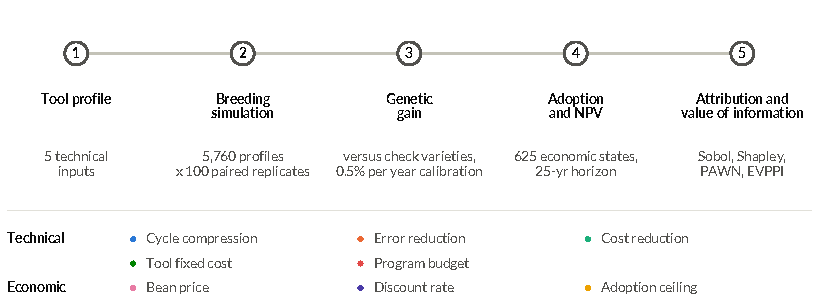
\includegraphics[width=\linewidth]{figures/fig1_design}
\caption{Study design. Each tool profile (five technical inputs) is simulated in a stochastic common-bean breeding program; its genetic gain over the check varieties is calibrated to realized progress, valued through variety adoption and discounting over the economic states, and attributed to its inputs. The colors identify the model inputs in all later figures.\label{fig:fig1_design}}
\end{figure}

\subsection{Case and Breeding Pipeline}
\label{sec:case}

The case is a public common-bean program in East Africa with a four-stage testing pipeline and a \NumCfgCycleYears{}-year cycle from cross to release. The stages are an observation nursery (ON), a preliminary yield trial (PYT), an advanced yield trial (AYT) and a national performance trial (NPT). The cycle length is an assumption of the model. A dry-bean simulation study used an eight-year cycle \cite{Lin2023Simulations}, and a CGIAR review notes that the path from a program decision to a widely grown variety, which includes adoption, rarely takes less than ten years \cite{Kholova2021Pursuit}. In this model $L$ is the time from cross to release, not the parent-recycling interval of the breeder's equation, and the adoption lag after release is modeled separately in Layer 2. Each cycle starts with \NumCfgNcrosses crosses among founders, each yielding \NumCfgNprogeny F1 plants, followed by \NumCfgNssd generations of single-seed descent to F5. The resulting F5 lines form the pool that enters the ON. Table~\ref{tab:inputs} lists lines, replicates, environments and selected fraction for each stage. These stage sizes are assumptions in the style of pipelines of the Pan-Africa Bean Research Alliance (PABRA), not values reported by a single source. The NPT selects \NumCfgNreleased lines for release.

Yield is simulated as a single additive polygenic trait on the \NumCfgNchr{} chromosomes of the common-bean genome \cite{Schmutz2014Reference}. The founder population has \NumCfgNfounders individuals, \NumCfgSegSites segregating sites per chromosome and \NumCfgQTLperChr quantitative trait loci (QTL) per chromosome, and the QTL number is an assumption. Mean yield is \NumCfgMeanYield{} kg/ha, consistent in order of magnitude with national average yields reported for African bean-growing countries \cite{Beebe2013Phenotyping} and with the average reported for Tanzania \cite{Hillocks2006Phaseolus}. The additive genetic standard deviation of the founders is \NumCfgSigmaA{} kg/ha, an assumption whose absolute scale the calibration removes (Section~\ref{sec:calibration}). Plot-level heritability of yield is \NumCfgHtwoYield{}, and the correlation that parameterizes genotype-by-environment interaction (GxE) between on-station environments is \NumCfgGxEOnstation. No source reports either value for this pipeline, so both are assumptions that a robustness block varies (Section~\ref{sec:inputs}).

\subsection{Layer 1: Stochastic Breeding Simulation}
\label{sec:layer1}

Each breeding cycle was simulated in AlphaSimR \cite{Gaynor2020Alphasimr}, with founder haplotypes from its coalescent simulator, for a manual program and a tool program in every replicate. Both programs share one founder population per replicate. Random founder pairs, drawn without replacement for each cross, produce F1 plants that are advanced to F5 by selfing. The four stages then apply truncation selection on phenotype, and a random subsample enters a stage when more lines are available than its size. AlphaSimR serves the strategic design of CGIAR-type programs with replicated stochastic runs \cite{Seck2024Stochastic,Gorjanc2018Optimal,FritscheNeto2023Improving}. Haplotype generation is not controlled by the R random-number seed, so a single replicate cannot be replayed in isolation.

Each stage selects on one phenotype per line, whose error variance gives the heritability of a genotype mean over the stage's replicates and environments. Let $\sigma^2_A$ be the genetic variance of the selection target and let GxE variance be parameterized as $\sigma^2_{GE} = (1-\rho_{GE})\,\sigma^2_A$, which is the parameterization implemented in the simulation. Then
\begin{equation}
h^2_{\mathrm{eff}} = \left[\, 1 + \frac{1-\rho_{GE}}{e} + \frac{1-h^2}{h^2\, r\, e} \,\right]^{-1},
\label{eq:heff}
\end{equation}
where $h^2$ is plot-level heritability, $r$ the number of replicates and $e$ the number of environments. Under the common variance-component definition of the genetic correlation between environments, $\rho = \sigma^2_A/(\sigma^2_A+\sigma^2_{GE})$, the same GxE variance corresponds to $\rho = 1/(2-\rho_{GE})$, so $\rho_{GE}$ is a parameter of this model and not a measured genetic correlation. The error variance of the single phenotype is
\begin{equation}
\sigma^2_{\varepsilon} = V_{\mathrm{ref}} \left( \frac{1}{h^2_{\mathrm{eff}}} - 1 \right),
\label{eq:vare}
\end{equation}
where $V_{\mathrm{ref}}$ is the genetic variance of the F5 pool entering the ON, computed once per program run. Plot error therefore stays constant across stages while selection depletes genetic variance, so realized heritability falls from stage to stage, whereas $h^2_{\mathrm{eff}}$ keeps its meaning on the F5-line basis. The tool's error reduction $\delta$ scales the single-plot error variance by $(1-\delta)$ before averaging over replicates and environments. With the single-plot error variance normalized to one, $\sigma^2_A = h^2/(1-h^2)$, and the tool program replaces $h^2$ in Equation~(\ref{eq:heff}) by
\begin{equation}
h^2_{\mathrm{tool}} = \frac{\sigma^2_A}{\sigma^2_A + (1-\delta)}.
\label{eq:htool}
\end{equation}
The genotype-by-environment term is unchanged by the tool, and $\delta$ may be negative for a tool noisier than manual scoring.

Genetic gain is the mean true genetic value of the released lines minus that of the check varieties, taken as the top $k$ founders, with $k$ equal to the number of released lines. The checks stand in for the elite varieties that farmers already grow. The gain over the founder mean is kept as a secondary output. For the manual program it averages \NumDGvsBaseTradPerCycle{} kg/ha per cycle across profiles, against \NumDGtradPerCycle{} kg/ha over the checks (both uncalibrated), so the check baseline is the more conservative reference. Both programs use common random numbers. Within a replicate they start from the same founder population, and the generator is re-seeded with the same pipeline seed immediately before each program runs. Crosses and generation advance are therefore identical, and noise largely cancels in the paired difference. Annual gain is the per-cycle gain divided by the cycle length, $L$ for the manual program and $L-c$ for the tool program with cycle compression $c$. A tool's advantage is expressed as the per-cycle uplift $u = 100\,\bar{D}/\bar{G}_{\mathrm{man}}$ (mean paired difference over mean manual gain), the annual uplift $100\,[(1+u/100)\,L/(L-c) - 1]$, and the equivalent compression $L - L/(1+u/100)$, the years of compression that raise annual gain by the same percentage as $u$. Figure~\ref{fig:fig2_time_beats_accuracy}b applies the last conversion to the mean per-cycle uplift of each robustness setting, averaged over its cost-reduction and compression levels, so the exchange rate includes the effect of cost reduction.

Both programs spend the same total budget per cycle, so a cheaper plot or a fixed tool cost changes how many lines and environments can be tested. Trial cost is the sum over stages of lines $\times$ environments $\times$ replicates $\times$ cost per plot, plus the tool fixed cost, which is zero for the manual program. The manual cost per plot is USD \NumCfgCostPerPlot, an assumption that also appears in \cite{Juliana2018Integrating} and is consistent in order of magnitude with East African costing \cite{Das2025Costing}. The tool's cost per plot is the manual cost multiplied by $(1-\text{cost reduction})$. A grid search varies PYT size from \NumCfgPYTmin{} to \NumCfgPYTmax{} lines in steps of \NumCfgPYTstep{} and PYT environments from one to \NumCfgPYTenvMax{}. The ON size is \NumCfgONmult{} times the PYT size, capped at \NumCfgONcap{} lines and at the F5 pool (crosses times progeny per cross), and ON plots are single-replicate and single-environment. The AYT and NPT sizes stay at the values in Table~\ref{tab:inputs}. Among the allocations that fit the budget, the search selects the maximizer of the breeder's-equation approximation of annual gain \cite{Cobb2019Enhancing}, $\hat{G} = L^{-1}\sum_{s} i_s \sqrt{h^2_{\mathrm{eff},s}}\,\sigma_A$, where $i_s$ is the selection intensity implied by the selected fraction of stage $s$. The allocation is chosen once per program and tool profile and used in every replicate. It trades the number of entries against replication \cite{Lorenz2013Resource}.

\subsection{Tool Inputs and Sweep Design}
\label{sec:inputs}

A tool profile is defined by five technical inputs: measurement-error reduction, whole-plot cost reduction, cycle compression, tool fixed cost and program budget (Table~\ref{tab:inputs}). Error reduction is the fractional reduction of single-plot error variance, and cost reduction is the fractional reduction of whole-plot cost. The simulated trait is yield, which a smartphone tool does not measure, because grain is harvested and weighed. No source we read shows how an image-based measure would lower the error variance of plot yield, for example by covariate adjustment with image-derived stand counts, and that pathway is untested here. Error reduction is therefore an effective reduction in the error variance of the selection phenotype, and the meta-analytic evidence for it concerns trait-level measurement error (Section~\ref{sec:ma}). It is not a measured property of yield recording.

Cycle compression is the number of years by which the tool shortens the breeding cycle. It leaves the simulated selection unchanged, because stage sizes, replicates and error variance do not depend on it, and it acts through the cycle length that divides gain and through the timing of release and spending in Layer 2. The simulation therefore treats compression as a scenario and does not model how a tool would achieve it. A tool could shorten the cycle only by bringing forward a selection decision, for example when stage data arrive early enough to recycle parents sooner \cite{Seck2024Stochastic}. Where beans are grown in two seasons per year, as in the bimodal-rainfall areas of Rwanda, Uganda and parts of Tanzania, the smallest such step is half a year; parts of the region, including most of Ethiopia and southern Tanzania, have a single bean season \cite{Katungi2018Effect,Jha2023Characterizing,Hillocks2006Phaseolus}. The main grid uses whole years from zero to \NumCfgCycMax{} because Layer 2 runs on an annual step, and a seasonal check covers zero, \NumCfgSeasonMid{} and one year (Section~\ref{sec:robust}). We found no study that measured how far a phenotyping tool shortens a breeding cycle. Precedents exist for other cycle-shortening technologies in dry bean, maize and rice \cite{Lin2023Simulations,Chaingeni2025More,Katiyar2026Unified}. Fixed cost (equipment and training) and budget are in USD per cycle, and the fixed cost is paid from within the budget. The evidence-based profile has an error reduction of \NumCfgErrRedCentral{}\% and a cost reduction of \NumCfgCostRedCentral{}\% (Section~\ref{sec:ma}). The error reduction is the median of the heritability-pair route (\NumERhtwoMedian\%) rounded to the nearest ten percent, whereas route T1 and the converted route T2 give negative medians, so this central value is at the favorable end of the evidence. The lower end of the fixed-cost range lies above reported hardware costs \cite{Mwanje2026Digital,Whan2014Grainscan}, and its upper end assumes training and data management. The budget grid lies above the operating cost per cycle reported for single national programs, USD \NumNatCostMin{} to \NumNatCostMax{} for maize pipelines in Uganda, Zambia and Zimbabwe and rice pipelines in four countries \cite{Das2025Costing,Katiyar2026Unified}, and it brackets the average operating cost of public breeding programs in the United States reported in \cite{Chaingeni2025More}, which cites a 2020 survey. We therefore model a regional breeding network: the pipeline pools the evaluation capacity of several national programs, and the grid spans the combined budget of roughly \NumNetProgMin{} to \NumNetProgMax{} national programs at these costs. Bean area is summed over the same six countries, so benefits and costs refer to the same scope. The cost anchors come from maize and rice and stand in for bean, so the network budget remains an assumption; because the budget barely moves the attribution of value (Section~\ref{sec:res_measure}), the conclusions do not depend on where in this range a real network lies.

\begin{table}[H]
\caption{Model inputs, explored values, central values and sources. ``Assumption'' marks values set by the authors that no cited source reports; each is explored in the sensitivity analysis or removed by the calibration.\label{tab:inputs}}
\begin{adjustwidth}{-\extralength}{0cm}
\footnotesize
\setlength{\tabcolsep}{3pt}
\begin{tabularx}{\fulllength}{>{\raggedright\arraybackslash}p{3.9cm}>{\raggedright\arraybackslash}p{2.0cm}>{\raggedright\arraybackslash}p{3.2cm}>{\raggedright\arraybackslash}p{2.6cm}>{\raggedright\arraybackslash}X}
\toprule
\textbf{Input} & \textbf{Unit} & \textbf{Explored values} & \textbf{Central or baseline} & \textbf{Source or status}\\
\midrule
\multicolumn{5}{l}{\textit{Technical inputs of the tool}}\\
Measurement-error reduction & \% of plot error variance & \NumCfgErrRedRange & \NumCfgErrRedCentral & Heritability-pair route of MA2, rounded (Section~\ref{sec:ma}); compatible with zero; effective reduction in selection error\\
Whole-plot cost reduction & \% of whole-plot cost & \NumCfgCostRedRange & \NumCfgCostRedCentral & MA3 time saving times data-capture share of plot cost \cite{Reynolds2019Costefficient}; upper bound on the saving from data capture alone\\
Cycle compression & Years & \NumCfgCycRange & \NumCfgCycCompCentral & Scenario; no measured effect found; precedents \cite{Lin2023Simulations,Chaingeni2025More,Katiyar2026Unified}\\
Tool fixed cost & USD per cycle & \NumCfgFixCostRange & \NumCfgFixCostCentral & Assumption; lower end above reported hardware costs \cite{Mwanje2026Digital,Whan2014Grainscan}\\
Program budget & USD per cycle & \NumCfgBudgetRange & \NumCfgBudgetCentral & Assumption: regional network of about \NumNetProgMin{}--\NumNetProgMax{} national programs \cite{Das2025Costing,Katiyar2026Unified}\\
\midrule
\multicolumn{5}{l}{\textit{Genetic and pipeline inputs}}\\
Plot-level heritability of yield & Ratio & \NumCfgRobHtwoLevels & \NumCfgHtwoYield{} & Assumption\\
GxE parameter $\rho_{GE}$ between on-station environments & Ratio & \NumCfgRobGxELevels & \NumCfgGxEOnstation & Assumption; $\sigma^2_{GE}=(1-\rho_{GE})\sigma^2_A$\\
Additive genetic standard deviation & kg/ha & Not varied & \NumCfgSigmaA{} & Assumption; scale removed by calibration\\
Chromosomes; founders; segregating sites and QTL per chromosome & Count & Not varied & \NumCfgNchr; \NumCfgNfounders; \NumCfgSegSites; \NumCfgQTLperChr & Chromosomes \cite{Schmutz2014Reference}; founders, sites and QTL are assumptions\\
Mean yield & kg/ha & Not varied & \NumCfgMeanYield{} & Order of magnitude consistent with \cite{Beebe2013Phenotyping,Hillocks2006Phaseolus}\\
Cycle length & Years & Not varied & \NumCfgCycleYears{} & Assumption; an eight-year dry-bean cycle is used in \cite{Lin2023Simulations}\\
Crosses per cycle; progeny per cross; selfing generations & Count & Not varied & \NumCfgNcrosses; \NumCfgNprogeny; \NumCfgNssd & Assumption\\
ON: lines; replicates; environments; selected \% & Count; \% & Lines optimized under the budget (Section~\ref{sec:layer1}) & \NumCfgStageONLines; \NumCfgStageONReps; \NumCfgStageONEnvs; \NumCfgStageONSelFrac{} & Assumption; PABRA-style pipeline\\
PYT: lines; replicates; environments; selected \% & Count; \% & Lines and environments optimized under the budget & \NumCfgStagePYTLines; \NumCfgStagePYTReps; \NumCfgStagePYTEnvs; \NumCfgStagePYTSelFrac{} & Assumption; PABRA-style pipeline\\
AYT: lines; replicates; environments; selected \% & Count; \% & Not varied & \NumCfgStageAYTLines; \NumCfgStageAYTReps; \NumCfgStageAYTEnvs; \NumCfgStageAYTSelFrac{} & Assumption; PABRA-style pipeline\\
NPT: lines; replicates; environments; selected \% & Count; \% & Not varied & \NumCfgStageNPTLines; \NumCfgStageNPTReps; \NumCfgStageNPTEnvs; \NumCfgStageNPTSelFrac{} & Assumption; PABRA-style pipeline\\
Manual cost per plot & USD & Not varied & \NumCfgCostPerPlot & Assumption that also appears in \cite{Juliana2018Integrating}; order of magnitude consistent with \cite{Das2025Costing}\\
\midrule
\multicolumn{5}{l}{\textit{Calibration and economic inputs}}\\
Realized gain target & \% of mean yield per year & Not varied in the main analysis; \NumCfgTargetLow{} and \NumCfgTargetHigh{} in robustness scenarios & \NumGainTargetPct{} & MA1 (Section~\ref{sec:ma})\\
Bean price & USD/kg & \NumCfgPriceRange & \NumBasePrice{} & Assumption informed by the mean and range of farm-gate prices in Uganda \cite{Jjagwe2022Role}\\
Discount rate & \% & \NumCfgDiscRange & \NumBaseDisc{} & Rates in practice \cite{Harberger2015Musings,Groom2022Future}\\
Adoption ceiling & \% of bean area & \NumCfgAdoptRange & \NumBaseAdopt{}\textsuperscript{a} & Levels consistent with \cite{Alene2019Measuring,Spielman2019Policy}; a modeling choice\\
Bean area & Million ha & \NumCfgAreaRange & \NumBaseArea{} & Brackets FAOSTAT area harvested \cite{FAO2025FAOSTATQCL}\\
Logistic rate; midpoint & Per year; years & Not varied in the main analysis; rate \NumCfgKLow{} and \NumCfgKMid{} in robustness scenarios & \NumCfgDiffK; \NumCfgDiffMid & Assumption; observed pace \cite{Alene2019Measuring}\\
Evaluation horizon & Years & Not varied in the main analysis; \NumCfgHorizonLong{} in a robustness scenario & \NumCfgHorizon{} & Common in ex ante work \cite{Staver2020ExAnte}\\
Tool running cost (net-value scenarios only) & Million USD per year & \NumCfgRunCostLow, \NumCfgRunCostMid{} and \NumCfgRunCostHigh & Not in the main NPV & Assumption; the order of magnitude of a global system is ``a few million USD per year'' \cite{Lasdun2024Participatory}\\
\bottomrule
\end{tabularx}
\end{adjustwidth}
\noindent{\footnotesize{\textsuperscript{a} The configured central adoption ceiling lies midway between two grid levels, and the baseline state takes the lower level.}}
\end{table}

The main grid and two extension blocks form one full factorial design of \NumNcellsOK{} tool profiles (\NumNgridTech{} combinations of error reduction, cost reduction, fixed cost and budget at each of four compression levels), each simulated with \NumNrepsPerCell{} paired replicates. The main grid crosses five levels of error reduction, five of cost reduction, four of cycle compression, six of fixed cost and five of budget (\NumNcellsMain). Extension A adds an error reduction of zero across eight levels of cost reduction, because the agreement evidence in MA2 is compatible with no improvement over manual scoring (\NumNcellsExtA). Extension B adds the lower whole-plot cost reductions implied by MA3 for the positive error reductions (\NumNcellsExtB). The union has six levels of error reduction and eight of cost reduction. The mean standard error of the paired per-cycle difference is \NumDGdiffSE{} kg/ha (uncalibrated). A stress block of \NumNcellsStress{} further profiles was simulated at zero compression with an error reduction of \NumCfgStressErr\%, that is, a tool noisier than manual scoring, at the lowest and the central cost reduction, the central fixed cost and three budgets; because compression leaves the selection unchanged, Layer 2 reuses these gains at every compression level. The stress block is not part of the main lookup table. Simulations ran on the Rorqual cluster of Calcul Qu\'ebec and the Digital Research Alliance of Canada.

Because no source reports plot-level heritability or the on-station GxE parameter for this pipeline, a separate robustness block varies both on a reduced tool grid. It crosses three levels of heritability (\NumCfgRobHtwoLevels) and three of the GxE parameter (\NumCfgRobGxELevels) with five levels of error reduction (zero to the maximum), three of cost reduction and four of cycle compression, at the baseline fixed cost and budget. It comprises \NumNcellsRobust profiles with \NumNrepsPerCell{} replicates each. The block feeds Figures~\ref{fig:fig2_time_beats_accuracy}b and \ref{fig:fig3_gain_ceiling}c only and is not part of the economic lookup table.

\subsection{Calibration of Simulated Gain to Realized Progress}
\label{sec:calibration}

We rescaled simulated gain by one common factor so that the manual program's mean annual gain equals realized progress in common-bean breeding. Averaged over all profiles, the simulated manual program gains \NumDGtradPerYear{} kg/ha per year over the checks, or \NumDGtradPctPerYearRaw\% of mean yield per year, which exceeds the realized rate. The target is \NumGainTargetPct{}\% per year of the mean yield of \NumCfgMeanYield{} kg/ha, the pooled realized gain of common-bean programs in MA1 (Section~\ref{sec:ma}). Three of the four programs in MA1 are Brazilian, the East African PABRA estimates alone are about 0.5\% per year \cite{Amongi2023Gain}, and the confidence interval of the pooled estimate reaches zero. Public programs that serve smallholders realize well under one percent annually \cite{Cobb2019Enhancing}. The factor of \NumGainScale{} multiplies the manual gain, the tool gain and the paired difference of every profile, and gives a calibrated manual gain of \NumDGtradPerYearCal{} kg/ha per year. Relative per-cycle uplifts are unchanged by this step, and money values shrink. NPV is not proportional to the factor, because the program budget in the cash flow is not rescaled. Gain is proportional to the additive genetic standard deviation in the breeder's-equation approximation of this model, so the common factor is equivalent to setting that standard deviation to \NumGainScale{} of its assumed value. A calibration through lower plot-level heritability or a lower GxE parameter would instead change relative uplifts, but the simulated manual program gains \NumRobManualGainPctMin{} to \NumRobManualGainPctMax{} percent of mean yield per year across the robustness block, at least \NumRobManualGainFoldMin{} times the target, so heritability within the explored range cannot close the gap. If real programs gain slowly because their effective heritability is below the explored range, accuracy would carry more value than we report, and we did not run that case, which needs Layer 1 simulations at lower heritability. We tested the calibration target at \NumCfgTargetLow{} and \NumCfgTargetHigh{}\% per year (Section~\ref{sec:robust}). Era-trial rates reflect decades of overlapping cycles, whereas the simulation covers one cycle, which adds to the uncertainty of the target.

\subsection{Layer 2: Adoption, Net Present Value and Equivalent Annual Value}
\label{sec:layer2}

The value of the tool is the net present value of its incremental cash flow over the manual program across a \NumCfgHorizon{}-year horizon $H$ (years zero to $H$). Let $L_j$ be the cycle length of program $j$, with $L_{\mathrm{man}} = L$ and $L_{\mathrm{tool}} = L-c$. Each program spends its budget evenly over the $L_j$ years of its cycle, so a shorter cycle spends the same budget sooner. The tool's fixed cost acts through the Layer 1 allocation and is not an additional cash flow, and the main NPV excludes the cost of developing, hosting and supporting the tool (Section~\ref{sec:robust} adds it as a scenario). Release occurs at the end of the cycle, in year $L_j$. From release, the yield advantage of the released lines over the check varieties builds at the annual gain $g_j = G_j/L_j$ until it equals the per-cycle gain $G_j$ after $L_j$ years, and then stays at $G_j$. The ramp is a modeling simplification: it lets the advantage build over one cycle length, as successive releases from overlapping cycles would, and then credits no further cycles. The benefit of program $j$ in year $t \geq L_j$ is
\begin{equation}
B^{j}_t = g_j\,\min(t-L_j+1,\,L_j)\; p\; a(t-L_j)\; A,
\label{eq:benefit}
\end{equation}
where $p$ is the bean price, $a(\cdot)$ the adoption rate and $A$ the bean area. The spending $C^{j}_t$ equals the budget divided by $L_j$ in years before release and zero afterwards. With $r$ the discount rate,
\begin{equation}
\mathrm{NPV} = \sum_{t=0}^{H} \frac{\left(B^{\mathrm{tool}}_t - B^{\mathrm{man}}_t\right) - \left(C^{\mathrm{tool}}_t - C^{\mathrm{man}}_t\right)}{(1+r)^{t}}.
\label{eq:npv}
\end{equation}
We use NPV rather than a benefit-cost ratio, which favors underinvestment \cite{Janssen2018Costbenefit}. The gains $G$ are the calibrated means over replicates for each profile. NPV therefore varies across tool profiles and economic states but not across replicates, so Monte Carlo variation within a profile does not enter the NPV distribution.

Adoption follows a logistic curve with a ceiling, the standard form in ex ante breeding evaluations \cite{Grovermann2022Three},
\begin{equation}
a(\tau) = \frac{K}{1 + \exp\left[-k\,(\tau - \tau_{\mathrm{mid}})\right]},
\label{eq:logistic}
\end{equation}
where $\tau$ is the time since release, $K$ the adoption ceiling, $k$ the rate and $\tau_{\mathrm{mid}}$ the midpoint. The ceiling is swept. The rate (\NumCfgDiffK) and the midpoint (\NumCfgDiffMid) are fixed assumptions in the main analysis. The assumed rate implies a faster gain in area than the roughly one percentage point per year observed for improved beans \cite{Alene2019Measuring}, so slower rates are tested in the robustness scenarios. The ceiling levels are consistent with a modern-variety share of about one third of bean area \cite{Alene2019Measuring} and a similar mean across African crops, which is reported secondhand \cite{Spielman2019Policy}.

Each tool profile was valued at every state of the full factorial of five levels of each of four economic inputs: bean price, discount rate, adoption ceiling and bean area. This design gives \NumNlookupRows{} profile-state combinations. The price levels span the mean farm-gate prices reported for Uganda (0.37 and 0.51 USD per kg) and extend above the observed maximum of 1.14 USD per kg, whereas the lowest level lies above the observed minimum of 0.20 USD per kg \cite{Jjagwe2022Role}. The discount-rate levels bracket the rates that Global South governments and development banks use \cite{Harberger2015Musings,Groom2022Future}. The area levels range from \NumCfgAreaRange{} million ha. They bracket the dry-bean area harvested in \NumFaoYearFrom{}--\NumFaoYearTo{}, which was \NumFaoSixMin{}--\NumFaoSixMax{} million ha summed over Uganda, Kenya, Tanzania, Rwanda, Burundi and Ethiopia and \NumFaoEAMin{}--\NumFaoEAMax{} million ha for the FAOSTAT region of Eastern Africa \cite{FAO2025FAOSTATQCL}. Area harvested counts land once per season, so in two-season areas it exceeds the physical bean area; the annual benefit per hectare in Layer 2 is defined on the same basis. The baseline state takes the grid point nearest the configured central values: a price of \NumBasePrice{} USD/kg, a discount rate of \NumBaseDisc{}\%, an adoption ceiling of \NumBaseAdopt{}\% and an area of \NumBaseArea{} million ha. The stressed state combines the lowest price, the highest discount rate, the lowest ceiling and the smallest area. In that state we also computed, for every pair of levels of two tool inputs, the median NPV over the remaining tool inputs (the break-even marginals). The equivalent annual value (EAV) per hectare converts NPV into a level annual stream over the horizon,
\begin{equation}
\mathrm{EAV} = \frac{\mathrm{NPV}\; r}{\left[1-(1+r)^{-H}\right] A}.
\label{eq:eav}
\end{equation}
Multiplying EAV by the area gives the level annual cost that the program could carry before NPV falls to zero, the break-even running cost.

\subsection{Global Sensitivity and Decision Analysis}
\label{sec:gsa}

The Layer 1 profiles and the economic levels form a full factorial grid. With area fixed at the baseline, the model is a table of NPV values over eight inputs (the five technical inputs plus price, discount rate and adoption ceiling), and every conditional expectation $\mathrm{E}[Y \mid X_S]$ of NPV $Y$ given a subset $S$ of inputs follows by exact averaging over the table (\NumNexactGrid{} values). All inputs take their simulated levels with equal probability, so one prior serves the variance attribution and the decision analysis. This replaces the sampling of continuous uniform inputs mapped to the nearest simulated profile, which gave the end levels half the weight of the interior levels. Area is fixed at the baseline in both analyses. First-order and total-order Sobol indices \cite{Sobol2001Global} follow from $S_i = \mathrm{Var}(\mathrm{E}[Y \mid X_i])/\mathrm{Var}(Y)$ and $S^T_i = 1 - \mathrm{Var}(\mathrm{E}[Y \mid X_{-i}])/\mathrm{Var}(Y)$. They are exact, so they carry no Monte Carlo error and no sample-size choice. A total-order index of zero is necessary and sufficient for an input to be non-influential \cite{Pianosi2016Sensitivity}. The remaining uncertainty is the noise in the Layer 1 gains. To gauge it, we added normal noise with the standard error of each profile's paired difference to the tool gain, recomputed the indices \NumBootB{} times and report the largest shift of any total-order index.

Three further measures test whether the ranking depends on the variance attribution or on input independence. Shapley effects \cite{Owen2017Shapley,Song2016Shapley,Iooss2019Shapley} were computed exactly as the average of the marginal contribution of each input over all orderings of the eight inputs, with the cost function $c(S) = \mathrm{Var}(\mathrm{E}[Y \mid X_S])$, for independent inputs and for a Gaussian copula discretized on the grid. For independent inputs, each Shapley effect must lie between the first-order and total-order indices \cite{Iooss2019Shapley}, which we verified for every input. The copula correlations are assumptions: positive for discount rate with price (correlation \NumCfgCopRhoPriceDisc), adoption ceiling with budget (\NumCfgCopRhoAdoptBudget) and compression with error reduction (\NumCfgCopRhoCycErr), and negative for cost reduction with fixed cost (\NumCfgCopRhoCostFix). The four pairs are disjoint, so the joint probability of a grid point is the product of four bivariate normal rectangle probabilities. PAWN \cite{Pianosi2015Simple} is the median Kolmogorov-Smirnov distance between the conditional distribution of NPV at each level of an input and its unconditional distribution, computed exactly on the grid. Its magnitude depends on the choice of summary statistic \cite{Puy2020Sensitivity}. Horizon-dependent total-order indices use the NPV truncated at each year from zero to \NumCfgHorizon{} with the same prior. Active subspaces \cite{Constantine2014Active} come from central finite-difference gradients at \NumCfgASN{} random points in normalized space, with a step of \NumCfgASstep{} in normalized units on each side, for the lookup mapped to the nearest simulated profile. Because that lookup is piecewise constant, a gradient differs from zero only where a step crosses a boundary between grid levels, so the eigenvalues depend on the step and on the spacing of the grid, and we use them as a qualitative check. The eigenvalues give shares of the mean squared gradient. Because each measure answers a different question, we compare rankings across measures, not magnitudes.

The expected value of perfect partial information (EVPPI) measures how much learning an input would be worth to a decision between investing in the tool and an alternative with a fixed payoff $\tau$, the hurdle \cite{Claxton2001Bayesian}. For input $X_i$,
\begin{equation}
\mathrm{EVPPI}_i(\tau) = \mathrm{E}_{X_i}\!\left[\max\left(\mathrm{E}[\mathrm{NPV}\mid X_i],\,\tau\right)\right] - \max\left(\mathrm{E}[\mathrm{NPV}],\,\tau\right).
\label{eq:evppi}
\end{equation}
We computed it exactly on the grid by conditioning on each level of each of the eight inputs, under the prior above. Three hurdles are used. The first is a multiple of the prior expected NPV (\NumEVprior{} million USD), from zero to \NumCfgHurdleMaxMult{} times that value; EVPPI peaks at the indifference hurdle $\tau = \mathrm{E}[\mathrm{NPV}]$ by construction, and no named alternative investment sets that value. The second is zero, the decision to invest in the tool or not. The third applies the zero hurdle to NPV net of an incremental annual running cost of \NumCfgRunCostLow, \NumCfgRunCostMid{} and \NumCfgRunCostHigh{} million USD paid in every year of the horizon, which makes the investment decision depend on the information. Conditioning on grid levels avoids the upward bias of nested Monte Carlo with small inner samples \cite{Brennan2007Calculating} and the regression step of single-sample estimators \cite{Strong2013Estimating,Heath2017Review}. An EVPPI above the cost of research is necessary but not sufficient for the research to be worthwhile \cite{Rothery2020Value}.

Expected NPV was also decomposed into a pessimistic corner, an optimistic corner and the remaining mixed states, over all profile-state combinations including area. The pessimistic corner has price, adoption ceiling and cycle compression at or below the lower tercile cut point of their distributions over the lookup table, and the discount rate at or above the upper cut point. With five levels per economic input and four levels of compression, this assigns the lowest two levels of price and ceiling, the highest two levels of discount rate, and zero or one year of compression to the corner. The optimistic corner is the mirror image. Because compression has four levels and none falls in the middle tercile, the remaining states form one mixed group, so three groups result. For each group we report the share of states, the mean and median NPV and the probability that NPV is negative.

\subsection{Robustness Analyses}
\label{sec:robust}

Each robustness analysis re-evaluates the exact NPV table under one changed assumption, without new Layer 1 simulation, and reports the same measures (expected NPV, total-order indices of compression and error reduction, and EVPPI at the indifference hurdle). Four analyses change the prior on cycle compression: levels zero and one year with equal weight; zero with probability \NumCfgZeroMassA{} and one to three years sharing the rest; zero with probability \NumCfgZeroMassB{} and one year with the rest; and seasonal steps of \NumCfgSeasonStep{} year with compression of zero, \NumCfgSeasonMid{} and one year, for which the gains of the four compression cells of each profile are pooled, because compression leaves selection unchanged. Five analyses change the economic structure: no ramp, so that the full per-cycle gain applies from release; recurrent cycles, in which the advantage keeps accruing each year without the cap and spending continues every year; a horizon of \NumCfgHorizonLong{} years; and adoption rates of \NumCfgKLow{} and \NumCfgKMid{}. A combination with no ramp, a rate of \NumCfgKLow{} and a horizon of \NumCfgHorizonLong{} years is also run with compression of zero or one year. Two analyses change the calibration target to \NumCfgTargetLow{} and \NumCfgTargetHigh{}\% per year. The running-cost scenarios subtract the annual cost above from the NPV. The no-ramp variant removes the faster ramp of the shorter cycle and so lowers the weight of compression. The recurrent-cycle variant credits more cycles to the shorter program and so raises it, and it bounds the simplification of the single-cycle model from the other side.

\subsection{Literature Searches and Meta-Analyses of Model Inputs}
\label{sec:ma}

Three meta-analyses grounded the model inputs. MA1 pools realized genetic gain in common bean, with other African staples as context. MA2 pools agreement between image-based or AI tools and manual references. MA3 pools time and cost savings of digital phenotyping. Candidate studies came from a federated search of OpenAlex, Semantic Scholar and Crossref that returned at most 25 records per query and source, supplemented for MA3 by direct queries of Crossref and Europe PMC. All searches ran on \NumSearchDate{}, with \NumPrismaOneQueries{}, \NumPrismaTwoQueries{} and \NumPrismaThreeQueries{} queries for MA1, MA2 and MA3 (query strings and hit counts in Supplementary Table S1). The searches identified \NumPrismaOneRecords{}, \NumPrismaTwoRecords{} and \NumPrismaThreeRecords{} records, of which \NumPrismaOneUnique{}, \NumPrismaTwoUnique{} and \NumPrismaThreeUnique{} remained after removing duplicates by DOI; reference lists and the other literature searches of this project contributed \NumPrismaOneOther{}, \NumPrismaTwoOther{} and \NumPrismaThreeOther{} further candidates. Of \NumPrismaOneSought{}, \NumPrismaTwoSought{} and \NumPrismaThreeSought{} reports sought, \NumPrismaOneAssessed{}, \NumPrismaTwoAssessed{} and \NumPrismaThreeAssessed{} were obtained legally and read in full, and \NumPrismaOneIncluded{}, \NumPrismaTwoIncluded{} and \NumPrismaThreeIncluded{} studies were included (flow diagrams in Supplementary Figure S1). Title and abstract screening was logged record by record only for MA2, where a title-keyword rule removed off-topic records; for MA1 and MA3 the number of records excluded at screening was not recorded. The MA1 pool rests on \NumMAoneKclus programs, so its prediction interval is indicative. A study entered a model only if it was marked as included, its DOI was verified against Crossref and re-checked live, and its full text had been read. Every extracted value carries its page or table locator. No formal risk-of-bias tool was applied. Table~\ref{tab:ma2appraisal} instead lists, for each MA2 effect, the crop, trait, platform, type of manual reference, unit of observation and preprint status. Some discovery queries timed out, so statements that no study was found refer to these searches only. Preprints stay in the primary sets and are removed in a sensitivity analysis. Topic searches on breeding simulation, phenotyping tools, breeding and adoption economics, and sensitivity and value-of-information methods also looked for a coupled breeding-simulation and adoption-economics valuation of a phenotyping tool, for global sensitivity analysis of a stochastic breeding simulation, and for value-of-information analysis of a breeding or phenotyping investment. We found none, and a re-run on \NumNoveltyDate{} with \NumNoveltyQueries{} queries in the federated search and in Crossref confirmed this; OpenAlex and Semantic Scholar were unavailable during the re-run because of rate limits, so it rests mainly on Crossref. The closest studies simulate phenotyping in breeding pipelines without adoption economics or value-of-information analysis \cite{Peixoto2023Simulationbased,Jahufer2021Deterministic,Lane2021High}.

All pooled estimates come from random-effects models fitted by REML in metafor, with three-level models where several effects share a program or study and Knapp-Hartung (t) intervals because the number of effects is small. For MA1, the effect is the regression slope divided by the era-trial mean, in percent of mean yield per year, with standard errors taken or derived from the source tables. For MA2, correlations were Fisher z-transformed with sampling variance $1/(n-3)$, where $n$ is the number of observation units of the effect (plots, plants, images, accessions, lines or cultivars; Table~\ref{tab:ma2appraisal}), and Spearman coefficients and square roots of $R^2$ were treated as Pearson correlations. Because the pooled correlation mixes traits, platforms and reference types with very high heterogeneity, it is descriptive, and the trait-specific estimates are the more meaningful summaries. Small-study checks (an Egger-type test, a rank test and trim-and-fill) were applied at the study level only. For MA3, the effect is the log ratio of time per unit of data, pooled without weights because no study reports a variance, so the random-effects model amounts to an unweighted t-interval, and back-transformed to a percent time reduction. We report 95\% prediction intervals next to confidence intervals, because they describe what a new program or tool might show. Sensitivity analyses used one effect per cluster, leave-one-out, exclusion of preprints and imputed standard errors. Pooled estimates are shown in Table~\ref{tab:meta}.

A tool-manual correlation does not identify error reduction, so we bounded it by three routes. Let $E = 1-\rho^2$ be the error share of a measurement, with $\rho$ its correlation with the true value, and $\mathrm{ER} = 1 - E_{\mathrm{tool}}/E_{\mathrm{manual}}$. Route T1 treats the manual reference as error-free, so that $\rho_{\mathrm{tool}}$ equals the pooled correlation. Route T2 treats the reference as a manual measure with independent errors, so that $\rho_{\mathrm{tool}}$ equals the pooled correlation divided by the correlation of manual scoring with the true value, $\rho_{\mathrm{manual}}$. The manual-reliability evidence (MA2b, three studies) contains three kinds of coefficient: correlations of a visual estimate with a digital measurement of the true severity, which estimate $\rho_{\mathrm{manual}}$ directly; correlations between two raters, which for parallel measures with independent errors equal $\rho_{\mathrm{manual}}^2$; and squared correlations between two ratings, which equal $\rho_{\mathrm{manual}}^4$. We pooled the coefficients as entered, which gives T2 as entered, and again after converting every row to $\rho_{\mathrm{manual}}$ by taking the square root of between-rater correlations and the fourth root of squared correlations, which gives T2 converted. Intra-rater repeatability also contains persistent rater bias, so the converted value is an upper bound on validity. We propagated the sampling uncertainty of the pooled correlations through T1 and both T2 variants by Monte Carlo (\NumMAtwoMCdraws{} draws) and discarded infeasible draws under T2. The third route uses heritability pairs, the ratio of noise to signal $(1-h^2)/h^2$ for image traits over manual traits. Whole-plot cost reduction is the data-capture (non-handling) share of plot cost, taken from a cost model for high-income phenotyping infrastructure and therefore an upper bound on the saving from data capture alone \cite{Reynolds2019Costefficient}, multiplied by the time saving of field handheld tools \cite{Walter2019Highthroughput,Lasdun2024Participatory}.

\subsection{Software and Reproducibility}
\label{sec:software}

The full chain from simulation summaries to every number in the text is scripted. Layer 1 was run on a computing cluster in R \NumRVersionHPC{} with AlphaSimR \NumAlphaSimRVersionHPC{} and data.table. Layer 2, the exact sensitivity and decision analyses, the robustness scenarios and the number export were run locally in R \NumRVersionLocal{} with data.table, arrow and mvtnorm. The meta-analyses ran in R \NumRVersionMA{} with metafor \NummetaforVersion{}. Figures were drawn in Python with matplotlib. A Makefile regenerates the Layer 2 outputs and the file of number macros, so every result number in the manuscript is a generated macro. The tables of meta-analysis results and the appraisal table are generated from the same files. Code and data availability: \TODO{repository URL and archive DOI}.

% Section 3: Results. Follows paper/outline.md, Section 3: one subsection per figure claim, Figures 2 to 6.
% Figure 1 (study design) belongs at the opening of Methods and is deliberately NOT placed here.
% Every result number is a \Num... macro from paper/numbers.tex (generated by paper/R/export_numbers.R).
\section{Results}\label{sec:results}

All results are simulated, ex ante and conditional on the explored ranges of the tool inputs, including zero to three years of cycle compression, which no study we found has measured and which the model applies as a scenario.

%==============================================================================
\subsection{Assumed Cycle Compression Separates Tool Profiles, and Accuracy Buys Months}\label{sec:res_time}

Years of cycle compression sort the annual genetic-gain uplift of the \NumNcellsOK\ simulated tool profiles into four groups, while measurement accuracy and plot cost spread profiles only within each group (Figure~\ref{fig:fig2_time_beats_accuracy}a). The separation follows from the model's arithmetic: one year of compression raises annual gain by \NumCycOneYearPct\% by construction, because the per-cycle gain is divided by a cycle of $L-1$ years instead of $L$. The median annual uplift over manual phenotyping was \NumAnnUpliftCycZero\% at zero compression and rose to \NumAnnUpliftCycOne\%, \NumAnnUpliftCycTwo\% and \NumAnnUpliftCycThree\% at one, two and three years. The interquartile ranges of the four groups (\NumAnnUpliftCycZeroQone\ to \NumAnnUpliftCycZeroQthree, \NumAnnUpliftCycOneQone\ to \NumAnnUpliftCycOneQthree, \NumAnnUpliftCycTwoQone\ to \NumAnnUpliftCycTwoQthree\ and \NumAnnUpliftCycThreeQone\ to \NumAnnUpliftCycThreeQthree\%) do not overlap, and the full ranges of adjacent groups overlap only in their tails. At zero compression, the uplift arises from accuracy and cost alone and averages \NumDGdiffPct\% per cycle across profiles.

\begin{figure}[H]
\begin{adjustwidth}{-\extralength}{0cm}
\centering
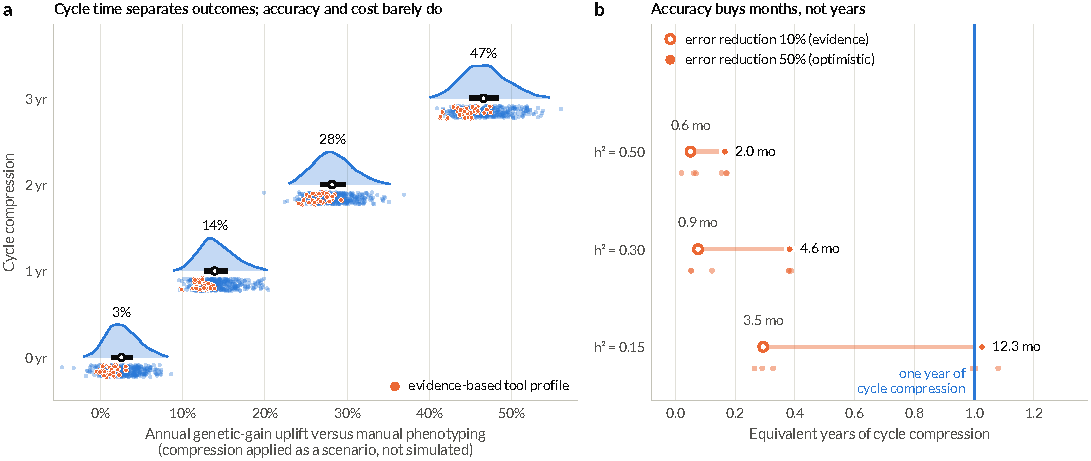
\includegraphics[width=\linewidth]{figures/fig2_time_beats_accuracy.pdf}
\end{adjustwidth}
\caption{Cycle time separates tool profiles, and accuracy buys months, not years. (\textbf{a}) Annual genetic-gain uplift over manual phenotyping across all simulated tool profiles, by years of cycle compression, which is applied as a scenario and not simulated (cloud: density; rain: profiles; bar and ring: interquartile range and median). Orange: evidence-based profile. (\textbf{b}) Exchange rate between accuracy and cycle time: years of breeding-cycle compression whose effect on annual genetic gain equals the tool's per-cycle uplift at the evidence-based and at the largest explored error reduction, by plot-level heritability (large markers: mean over the three on-station GxE parameter levels; small dots: individual settings). The uplift is averaged over the cost reductions of the robustness block and therefore includes their effect.\label{fig:fig2_time_beats_accuracy}}
\end{figure}

Accuracy gains within the range supported by the evidence are worth months, not years, of cycle compression (Figure~\ref{fig:fig2_time_beats_accuracy}b). In the robustness block, the per-cycle uplift at the evidence-based error reduction of \NumCfgErrRedCentral\% has the same effect on annual gain as \NumExchMoHtwoLowErrTen, \NumExchMoHtwoMidErrTen and \NumExchMoHtwoHighErrTen months of compression at the lowest, central and highest plot-level heritability (\NumCfgRobHtwoLow, \NumCfgHtwoYield\ and \NumCfgRobHtwoHigh). At the largest error reduction explored (\NumCfgErrRedMax\%), the equivalents are \NumExchMoHtwoLowErrFifty, \NumExchMoHtwoMidErrFifty and \NumExchMoHtwoHighErrFifty months. One full year of compression raises annual gain by \NumCycOneYearPct\%, a level that accuracy reaches only at the lowest heritability combined with the largest error reduction. Because the profiles that carry each error reduction also carry cost reductions, these equivalents overstate what accuracy alone buys.

The profile defined by the meta-analytic error and cost reductions draws almost all of its advantage from compression. This evidence-based profile (error reduction \NumCfgErrRedCentral\%, whole-plot cost reduction \NumCfgCostRedCentral\%) falls below the group median in every compression group (Figure~\ref{fig:fig2_time_beats_accuracy}a). Its median per-cycle uplift was \NumUpliftMeta\%, and its annual uplift was \NumAnnUpliftMetaCycZero\%, \NumAnnUpliftMetaCycOne\%, \NumAnnUpliftMetaCycTwo\% and \NumAnnUpliftMetaCycThree\% at zero to three years of compression.

%==============================================================================
\subsection{Accuracy and Cost Savings Move Per-Cycle Gain by a Few Percent}\label{sec:res_gain}

Per-cycle gain rises steadily with measurement-error reduction but stays below the annual-gain effect of one year of compression at the central heritability (Figure~\ref{fig:fig3_gain_ceiling}a). The mean paired per-cycle difference between the tool and the manual program rose from \NumDGdiffErrZero\ kg/ha at zero error reduction through \NumDGdiffErrTen, \NumDGdiffErrTwenty, \NumDGdiffErrThirty\ and \NumDGdiffErrForty\ kg/ha to \NumDGdiffErrFifty\ kg/ha at the largest reduction, against a manual gain of \NumDGtradPerCycle\ kg/ha per cycle (uncalibrated simulation units). In relative terms, the median uplift rose from \NumUpliftErrZero\% to \NumUpliftErrFifty\%, whereas one year of compression raises annual gain by \NumCycOneYearPct\%. Averaged over all profiles, the paired difference was \NumDGdiffPerCycle\ kg/ha (\NumDGdiffPct\% of the manual gain), with a mean Monte Carlo standard error of \NumDGdiffSE\ kg/ha. A negative mean difference occurred in \NumNcellsNegDiff\ of the \NumNcellsOK\ profiles, \NumNcellsNegDiffErrZero of them at zero error reduction. At zero error reduction the mean difference (\NumDGdiffErrZero\ kg/ha) is of the size of the standard error, so the sign of a single low-accuracy profile is partly Monte Carlo noise, and a tool fixed cost that neither accuracy nor cheaper plots offset can add to it.

\begin{figure}[H]
\centering
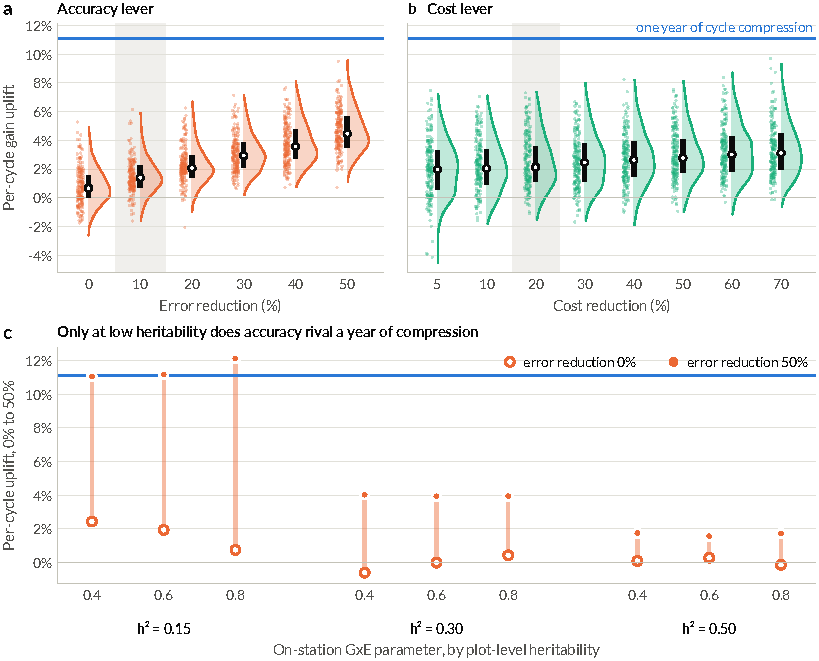
\includegraphics[width=\linewidth]{figures/fig3_gain_ceiling.pdf}
\caption{Accuracy and cost savings move per-cycle genetic gain by a few percent. (\textbf{a},\textbf{b}) Per-cycle genetic-gain uplift of the tool over manual phenotyping across all simulated tool profiles, by measurement-error reduction (\textbf{a}) and whole-plot cost reduction (\textbf{b}) ($h^2 = \NumCfgHtwoYield$; cloud: density; rain: profiles; bar and ring: interquartile range and median); shaded columns: evidence-based values. The vertical axes show the full range of the profiles, including negative uplifts. (\textbf{c}) Robustness: per-cycle uplift with no and with the largest error reduction for each combination of plot-level heritability and on-station GxE parameter. Blue lines: the annual-gain increase from one year of cycle compression.\label{fig:fig3_gain_ceiling}}
\end{figure}

Cheaper plots shift per-cycle uplift only modestly across their explored range (Figure~\ref{fig:fig3_gain_ceiling}b). Raising the whole-plot cost reduction from \NumCfgCostRedMin\% to \NumCfgCostRedMax\% moved the median per-cycle uplift from \NumUpliftCostFive\% to \NumUpliftCostSeventy\%. A fixed budget converts plot savings into more entries and environments, and selection gain shows diminishing returns to intensity and accuracy \cite{Cobb2019Enhancing}. The uplift was also larger at the smallest program budget (\NumUpliftBudgetLow\%) than at the largest (\NumUpliftBudgetHigh\%), a pattern consistent with a budget that limits trial size.

Only at the lowest plot-level heritability does the largest error reduction raise per-cycle gain to the level of one year of compression (Figure~\ref{fig:fig3_gain_ceiling}c). Averaged over the three GxE parameter levels, the per-cycle uplift at zero and at the largest error reduction was \NumRobUpliftHtwoLowErrZero\% and \NumRobUpliftHtwoLowErrFifty\% at the lowest heritability, \NumRobUpliftHtwoMidErrZero\% and \NumRobUpliftHtwoMidErrFifty\% at the central heritability, and \NumRobUpliftHtwoHighErrZero\% and \NumRobUpliftHtwoHighErrFifty\% at the highest. The one-year compression effect is \NumCycOneYearPct\%. At the central and highest heritability, the uplift stays well below that line at every GxE parameter level. Varying the on-station GxE parameter moved the uplift less than varying plot-level heritability did.

%==============================================================================
\subsection{Value Follows the Assumed Cycle Time}\label{sec:res_value}

The tool has a positive NPV in \NumPrNPVpos\% of the \NumNlookupRows\ profile-state combinations, and median NPV rises with each year of compression (Figure~\ref{fig:fig4_value_follows_time}a). Over all profiles and economic states, the median NPV was \NumNPVallCycZero million USD at zero compression and \NumNPVallCycThree million USD at three years. The evidence-based profile lay below the all-profile median at every compression level, at \NumNPVmetaCycZero and \NumNPVmetaCycThree million USD at zero and three years. Negative NPV occurred only at zero compression, and the number of negative values at one to three years was \NumNegNPVnonzeroComp.

\begin{figure}[H]
\begin{adjustwidth}{-\extralength}{0cm}
\centering
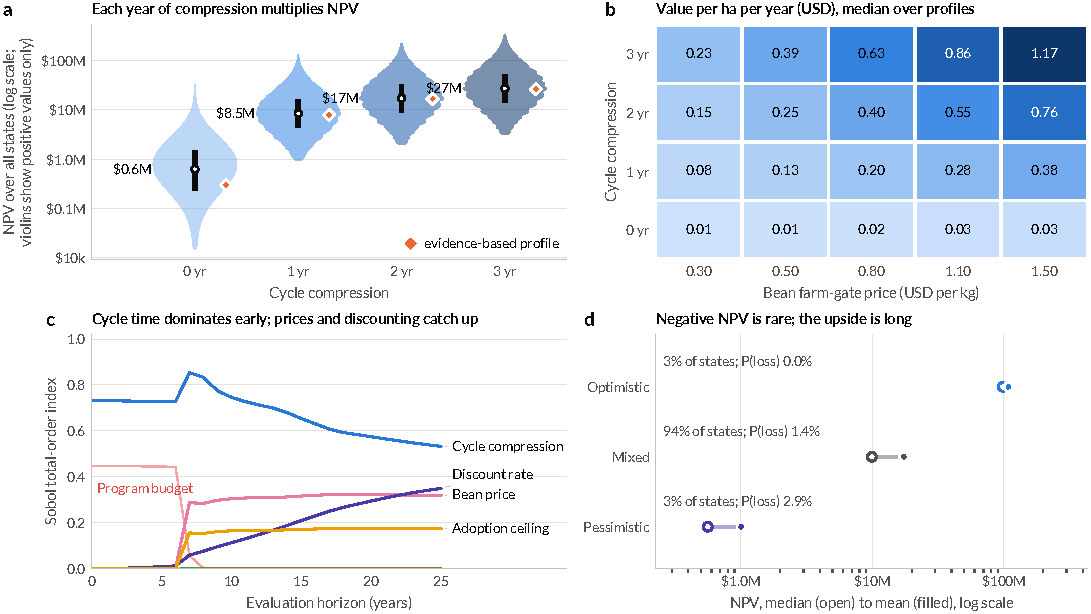
\includegraphics[width=\linewidth]{figures/fig4_value_follows_time.pdf}
\end{adjustwidth}
\caption{Value follows cycle time. (\textbf{a}) NPV of the tool across all tool profiles and economic states by cycle compression (violins of the positive values on a log scale; labels, bar and ring: median and interquartile range of all states; orange diamonds: median of the evidence-based profile). (\textbf{b}) Median equivalent annual value per hectare by cycle compression and bean price (discount rate \NumBaseDisc\%, adoption ceiling \NumBaseAdopt\%, bean area \NumBaseArea\ million ha). (\textbf{c}) Sobol total-order indices by evaluation horizon; the four inputs with the largest index at the final year and the program budget are labeled. (\textbf{d}) Median and mean NPV in the pessimistic and optimistic corners of the input space and in the remaining (mixed) states; P(loss): share of states with negative NPV.\label{fig:fig4_value_follows_time}}
\end{figure}

At the baseline economic state, the median equivalent annual value is small without compression and rises almost linearly with each year compressed (Figure~\ref{fig:fig4_value_follows_time}b). The baseline state has a bean price of \NumBasePrice\ USD/kg, a discount rate of \NumBaseDisc\%, an adoption ceiling of \NumBaseAdopt\% and a bean area of \NumBaseArea\ million ha. The median value was \NumEAAcycZero\ USD per hectare per year at zero compression and \NumEAAcycOne, \NumEAAcycTwo\ and \NumEAAcycThree\ USD per hectare per year at one, two and three years, or about \NumEAAperYearCompressed\ USD per hectare per year for each year compressed. The corresponding median NPV was \NumNPVcycZero, \NumNPVcycOne, \NumNPVcycTwo\ and \NumNPVcycThree\ million USD. NPV was positive in \NumPrPosCycZero\% of profiles at zero compression and in all profiles (\NumPrPosCycOne\%) at one, two and three years. Without compression, the value per hectare varied little across profiles (mean \NumConsEAAmean, standard deviation \NumConsEAAsd\ USD per hectare per year). Bean price raised the value within every row; at three years of compression, the median rose from \NumEAAcycThreePriceLow\ to \NumEAAcycThreePriceHigh\ USD per hectare per year between the lowest and highest price. These per-hectare values are small, and they become material only when summed over the \NumBaseArea\ million ha of the baseline state.

Median value stays positive in the most pessimistic economic state, and the dominance of compression is largest early in the horizon (Figure~\ref{fig:fig4_value_follows_time}c). In the state with the lowest price, highest discount rate, lowest adoption ceiling and smallest area (not shown in the figure), the median NPV across profiles was \NumStressMedianNPV\ million USD. For every tested pair of levels of two tool inputs, the median NPV over the remaining tool inputs in that state stayed positive (smallest value \NumStressMinMarginalNPV\ million USD). Before the first releases, NPV truncated at an evaluation year consists of incremental program costs, and it depends almost entirely on compression and program budget through the timing of spending. The total-order index of compression was \NumDynSTCycYearFive\ at year five, against \NumDynSTBudgetYearFive\ for program budget. It peaked at \NumDynSTCycPeak\ in year \NumDynSTCycPeakYear, the year of the earliest possible release, and declined to \NumDynSTCycFinal\ at year \NumCfgHorizon\ as discount rate, price and adoption ceiling gained weight.

Negative NPV is rare by construction, and the upside is concentrated in the optimistic corner (Figure~\ref{fig:fig4_value_follows_time}d). Both programs spend the same budget and tool costs replace plots within it, so NPV turns negative only where the simulated per-cycle gain difference is negative. The pessimistic corner (\NumScnPessimisticProb\% of states) had a mean NPV of \NumScnPessimisticMean\ and a median of \NumScnPessimisticMedian\ million USD, with \NumScnPessimisticPrNeg\% of states below zero. The mixed states (\NumScnOtherProb\%) had a mean of \NumScnOtherMean\ and a median of \NumScnOtherMedian\ million USD, with \NumScnOtherPrNeg\% below zero. The optimistic corner (\NumScnOptimisticProb\%) had a mean of \NumScnOptimisticMean\ and a median of \NumScnOptimisticMedian\ million USD, with \NumScnOptimisticPrNeg\% below zero. The mean exceeded the median in every group, which indicates right-skewed NPV distributions.

The main NPV excludes the cost of developing, hosting and supporting the tool. The median equivalent annual value multiplied by the area gives the level annual cost at which NPV falls to zero in the baseline state: \NumBECostCycZero, \NumBECostCycOne, \NumBECostCycTwo\ and \NumBECostCycThree\ million USD per year at zero to three years of compression. The only source we read on running cost puts a global AI phenotyping system at ``a few million USD per year'' \cite{Lasdun2024Participatory}, which exceeds the break-even cost at one year of compression and is of the same order as that at three years. Table~\ref{tab:netvalue} subtracts illustrative annual costs from the NPV. At \NumCfgRunCostLow\ million USD per year, the break-even compression was \NumBECompCostLow\ years, the expected net NPV was \NumRvEVCostLow\ million USD and it was positive in \NumRvPrPosCostLow\% of states. At \NumCfgRunCostHigh\ million USD per year, it was \NumRvEVCostHigh\ million USD and positive in \NumRvPrPosCostHigh\% of states, and the baseline-state median stayed negative at three years of compression (\NumRvNPVCycThreeCostHigh\ million USD).

\begin{table}[H]
\caption{Value of the tool net of an incremental running cost paid in every year of the horizon. Expected net NPV and the share of states with positive net NPV are over all tool profiles and economic states of the exact grid (bean area at the baseline). Break-even compression is the compression at which the median equivalent annual value at the baseline state, multiplied by the area, equals the running cost (linear interpolation between whole years). Median NPV is at the baseline economic state. EVPPI is at a decision hurdle of zero (invest or not).\label{tab:netvalue}}
\begin{adjustwidth}{-\extralength}{0cm}
\footnotesize
\setlength{\tabcolsep}{3pt}
\begin{tabularx}{\fulllength}{>{\raggedright\arraybackslash}X>{\centering\arraybackslash}p{1.4cm}>{\centering\arraybackslash}p{1.5cm}>{\centering\arraybackslash}p{1.6cm}>{\centering\arraybackslash}p{1.6cm}>{\centering\arraybackslash}p{1.6cm}>{\centering\arraybackslash}p{1.6cm}>{\centering\arraybackslash}p{1.4cm}>{\centering\arraybackslash}p{1.4cm}>{\centering\arraybackslash}p{1.5cm}}
\toprule
\textbf{Running cost (million USD per year)} & \textbf{Expected NPV} & \textbf{Share positive (\%)} & \textbf{Break-even compression (years)} & \textbf{Median NPV, 1 year} & \textbf{Median NPV, 3 years} & \textbf{EVPPI, compression} & \textbf{EVPPI, discount rate} & \textbf{EVPPI, price} & \textbf{EVPPI, error reduction}\\
\midrule
None (main analysis) & \NumRvEVBase & \NumRvPrPosBase & -- & \NumRvNPVCycOneBase & \NumRvNPVCycThreeBase & \NumEVPPIzeroHurdleMax & \NumEVPPIzeroHurdleMax & \NumEVPPIzeroHurdleMax & \NumEVPPIzeroHurdleMax\\
\NumCfgRunCostLow & \NumRvEVCostLow & \NumRvPrPosCostLow & \NumBECompCostLow & \NumRvNPVCycOneCostLow & \NumRvNPVCycThreeCostLow & \NumRvEVPPIzeroCycCostLow & \NumRvEVPPIzeroDiscCostLow & \NumRvEVPPIzeroPriceCostLow & \NumRvEVPPIzeroErrCostLow\\
\NumCfgRunCostMid & \NumRvEVCostMid & \NumRvPrPosCostMid & \NumBECompCostMid & \NumRvNPVCycOneCostMid & \NumRvNPVCycThreeCostMid & \NumRvEVPPIzeroCycCostMid & \NumRvEVPPIzeroDiscCostMid & \NumRvEVPPIzeroPriceCostMid & \NumRvEVPPIzeroErrCostMid\\
\NumCfgRunCostHigh & \NumRvEVCostHigh & \NumRvPrPosCostHigh & \NumBECompCostHigh & \NumRvNPVCycOneCostHigh & \NumRvNPVCycThreeCostHigh & \NumRvEVPPIzeroCycCostHigh & \NumRvEVPPIzeroDiscCostHigh & \NumRvEVPPIzeroPriceCostHigh & \NumRvEVPPIzeroErrCostHigh\\
\bottomrule
\end{tabularx}
\end{adjustwidth}
\end{table}

A tool noisier than manual scoring shows the downside that the main grid lacks. The stress block (error reduction \NumCfgStressErr\%, \NumNcellsStress\ profiles) changed per-cycle gain by \NumStressUpliftPct\% on average, with profiles between \NumStressDiffMin\% and \NumStressDiffMax\%, a pattern consistent with a lower cost per plot and a reallocated budget offsetting part of the added noise. At zero compression the median NPV was \NumStressNPVCycZero\ million USD, and NPV was positive in \NumStressPrPosCycZero\% of states. At one year of compression, the median NPV was \NumStressNPVCycOne\ million USD and positive in \NumStressPrPosCycOne\% of states, so the assumed time saving outweighed the added noise in this model.

%==============================================================================
\subsection{What a Pilot Should Measure}\label{sec:res_measure}

Cycle compression accounts for the largest share of NPV variance, followed by discount rate, price and adoption ceiling (Figure~\ref{fig:fig5_what_to_measure}a). The first-order and total-order Sobol indices were \NumSobolSoneCyc\ and \NumSobolSTCyc\ for compression, \NumSobolSoneDisc\ and \NumSobolSTDisc\ for discount rate, \NumSobolSonePrice\ and \NumSobolSTPrice\ for price, and \NumSobolSoneAdopt\ and \NumSobolSTAdopt\ for adoption ceiling. The total-order indices of the other four technical inputs (error reduction, cost reduction, program budget and tool fixed cost) were \NumSobolSTErrRed, \NumSobolSTCostRed, \NumSobolSTBudget\ and \NumSobolSTFixCost, respectively, so these inputs add almost nothing to NPV variance over the explored ranges \cite{Pianosi2016Sensitivity}. The indices are exact on the grid, and adding Layer 1 simulation noise of the size of the standard error of each profile's paired difference moved no total-order index by more than \NumSobolBootMaxShift. The first-order indices sum to \NumSobolSumSone\ and the total-order indices to \NumSobolSumST, so interactions carry the remainder of the variance, as expected for an NPV that multiplies gain, price, adoption and area.

\begin{figure}[H]
\centering
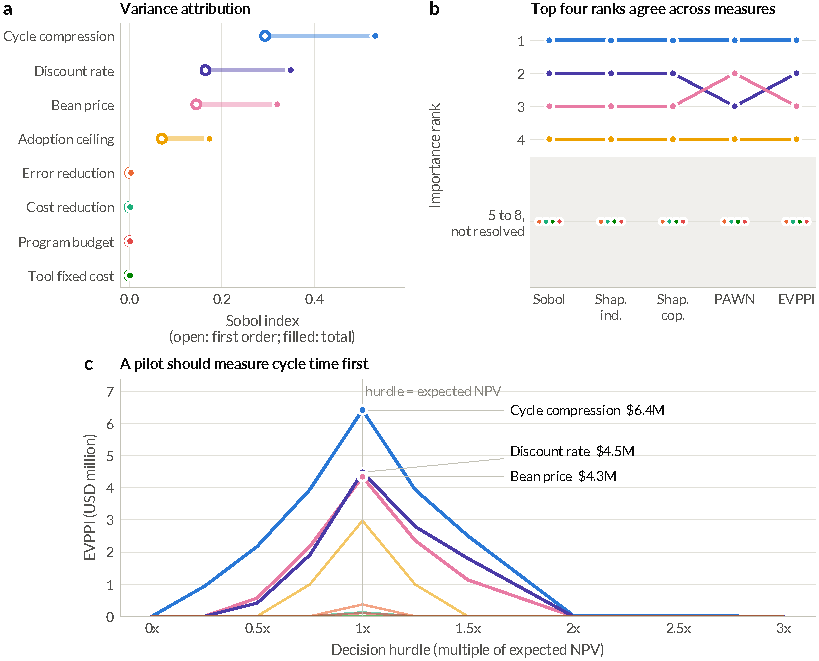
\includegraphics[width=\linewidth]{figures/fig5_what_to_measure.pdf}
\caption{What a pilot should measure. (\textbf{a}) First-order (open) and total-order (filled) Sobol indices of NPV. (\textbf{b}) Importance ranks of the inputs under five measures: Sobol total-order index, Shapley effects with independent and copula-correlated inputs, PAWN median, and EVPPI at the indifference hurdle; the four minor technical inputs (dots in the shaded band, colors as in panel a) lie below every other input on every measure, and their order is not resolved. (\textbf{c}) Expected value of perfect partial information (EVPPI) of each input as the payoff of the alternative investment varies (multiple of expected NPV); labels give the three largest values at the indifference point.\label{fig:fig5_what_to_measure}}
\end{figure}

When compression is fixed at zero, error reduction becomes the second-largest source of a much smaller NPV variance. The total-order indices were \NumSobolCycZeroSTDisc\ for discount rate, \NumSobolCycZeroSTErrRed\ for error reduction, \NumSobolCycZeroSTPrice\ for price, \NumSobolCycZeroSTBudget\ for program budget, \NumSobolCycZeroSTCostRed\ for cost reduction, \NumSobolCycZeroSTAdopt\ for adoption ceiling and \NumSobolCycZeroSTFixCost\ for tool fixed cost. Accuracy therefore matters for the residual value, which is small in absolute terms (Section~\ref{sec:res_value}). At the baseline economic state and zero compression, raising error reduction from zero to \NumCfgErrRedMax\% raised the median NPV from \NumRvNPVErrZero\ to \NumRvNPVErrFifty\ million USD, whereas one year of compression with no error reduction gave \NumRvNPVCycOneErrZero\ million USD.

Cycle compression ranks first under all five importance measures. Discount rate and price share ranks two and three, with their order depending on the measure, adoption ceiling ranks fourth on every measure, and the four minor technical inputs lie below all of them, with an order that is not resolved (Figure~\ref{fig:fig5_what_to_measure}b). Shapley effects with correlated inputs were \NumShapleyCyc\ for compression, \NumShapleyDisc\ for discount rate, \NumShapleyPrice\ for price, \NumShapleyAdopt\ for adoption ceiling, \NumShapleyErrRed\ for error reduction, \NumShapleyBudget\ for program budget, \NumShapleyCostRed\ for cost reduction and \NumShapleyFixCost\ for tool fixed cost. With independent inputs, the Shapley effects of compression, discount rate, price and adoption ceiling were \NumShapleyIndepCyc, \NumShapleyIndepDisc, \NumShapleyIndepPrice\ and \NumShapleyIndepAdopt, and those of error reduction and cost reduction were \NumShapleyIndepErrRed\ and \NumShapleyIndepCostRed. All \NumShapleyBracketN\ independent-input effects lie between the first-order and total-order indices of their input. PAWN gave \NumPawnCyc\ for compression, \NumPawnPrice\ for price, \NumPawnDisc\ for discount rate and \NumPawnAdopt\ for adoption ceiling, against \NumPawnErrRed, \NumPawnBudget, \NumPawnCostRed\ and \NumPawnFixCost\ for the four minor technical inputs. The first active-subspace direction of the lookup mapped to the nearest simulated profile carried \NumASshareOne\% of the mean squared gradient and the first two directions \NumAScumTwo\%. The first direction loads mainly on cycle compression (\NumASloadCycOne) and the second mainly on the economic inputs. Shapley effects sum to one, whereas the total-order Sobol indices sum to \NumSobolSumST, so rankings rather than magnitudes are compared across measures \cite{Iooss2019Shapley,Puy2020Sensitivity}.

The ranking survived every change we made to the assumptions that favor compression (Table~\ref{tab:robust}). In all \NumRvNscenarios\ scenarios, compression kept the first rank on the total-order index, with indices between \NumRvSTCycMin\ and \NumRvSTCycMax, against \NumRvSTErrMin\ to \NumRvSTErrMax\ for error reduction, and the smallest ratio of the two indices was \NumRvRatioMin. Restricting compression to zero or one year left the total-order index of compression at \NumRvSTCycPriorZeroOne\ against \NumRvSTErrPriorZeroOne\ for error reduction, and seasonal steps of zero, \NumCfgSeasonMid\ and one year gave \NumRvSTCycPriorSeason\ against \NumRvSTErrPriorSeason. Putting probability \NumCfgZeroMassB\ on no compression raised the index of compression to \NumRvSTCycPriorZeroHeavy. Removing the ramp, adding recurrent cycles, extending the horizon to \NumCfgHorizonLong\ years or slowing adoption changed the index between \NumRvSTCycHorizonForty\ and \NumRvSTCycRecurrent. The combination of no ramp, a slow rate and a long horizon with compression of zero or one year was the least favorable to compression, with indices of \NumRvSTCycConservativeZeroOne\ against \NumRvSTErrConservativeZeroOne. The calibration target changed expected NPV from \NumRvEVTargetQuarter\ million USD at \NumCfgTargetLow\% per year to \NumRvEVTargetOne\ million USD at \NumCfgTargetHigh\% per year, but it left the total-order indices of compression and error reduction unchanged to the printed precision.

\begin{table}[H]
\caption{Robustness of the attribution and decision results to the prior on cycle compression, the economic structure and the calibration target. Expected NPV (million USD) and total-order Sobol indices are over the exact grid with bean area at the baseline; EVPPI (million USD) is at the indifference hurdle, the expected NPV of each scenario.\label{tab:robust}}
\begin{adjustwidth}{-\extralength}{0cm}
\footnotesize
\setlength{\tabcolsep}{3pt}
\begin{tabularx}{\fulllength}{>{\raggedright\arraybackslash}X>{\centering\arraybackslash}p{2.0cm}>{\centering\arraybackslash}p{2.4cm}>{\centering\arraybackslash}p{2.4cm}>{\centering\arraybackslash}p{2.4cm}>{\centering\arraybackslash}p{2.4cm}}
\toprule
\textbf{Scenario} & \textbf{Expected NPV} & \textbf{Total index, compression} & \textbf{Total index, error reduction} & \textbf{EVPPI, compression} & \textbf{EVPPI, error reduction}\\
\midrule
\multicolumn{6}{l}{\textit{Prior on cycle compression}}\\
Equal weight on zero to three years (main analysis) & \NumRvEVBase & \NumRvSTCycBase & \NumRvSTErrBase & \NumRvEVPPICycBase & \NumRvEVPPIErrBase\\
Zero or one year, equal weight & \NumRvEVPriorZeroOne & \NumRvSTCycPriorZeroOne & \NumRvSTErrPriorZeroOne & \NumRvEVPPICycPriorZeroOne & \NumRvEVPPIErrPriorZeroOne\\
Zero, \NumCfgSeasonMid{} or one year (half-year steps) & \NumRvEVPriorSeason & \NumRvSTCycPriorSeason & \NumRvSTErrPriorSeason & \NumRvEVPPICycPriorSeason & \NumRvEVPPIErrPriorSeason\\
Zero with probability \NumCfgZeroMassA, one to three years share the rest & \NumRvEVPriorZeroMass & \NumRvSTCycPriorZeroMass & \NumRvSTErrPriorZeroMass & \NumRvEVPPICycPriorZeroMass & \NumRvEVPPIErrPriorZeroMass\\
Zero with probability \NumCfgZeroMassB, one year with the rest & \NumRvEVPriorZeroHeavy & \NumRvSTCycPriorZeroHeavy & \NumRvSTErrPriorZeroHeavy & \NumRvEVPPICycPriorZeroHeavy & \NumRvEVPPIErrPriorZeroHeavy\\
\midrule
\multicolumn{6}{l}{\textit{Economic structure}}\\
No ramp: full per-cycle gain from release & \NumRvEVRampStep & \NumRvSTCycRampStep & \NumRvSTErrRampStep & \NumRvEVPPICycRampStep & \NumRvEVPPIErrRampStep\\
Recurrent cycles with continued spending & \NumRvEVRecurrent & \NumRvSTCycRecurrent & \NumRvSTErrRecurrent & \NumRvEVPPICycRecurrent & \NumRvEVPPIErrRecurrent\\
Horizon of \NumCfgHorizonLong{} years & \NumRvEVHorizonForty & \NumRvSTCycHorizonForty & \NumRvSTErrHorizonForty & \NumRvEVPPICycHorizonForty & \NumRvEVPPIErrHorizonForty\\
Adoption rate \NumCfgKLow & \NumRvEVKTen & \NumRvSTCycKTen & \NumRvSTErrKTen & \NumRvEVPPICycKTen & \NumRvEVPPIErrKTen\\
Adoption rate \NumCfgKMid & \NumRvEVKFifteen & \NumRvSTCycKFifteen & \NumRvSTErrKFifteen & \NumRvEVPPICycKFifteen & \NumRvEVPPIErrKFifteen\\
No ramp, rate \NumCfgKLow, horizon \NumCfgHorizonLong{} years & \NumRvEVConservative & \NumRvSTCycConservative & \NumRvSTErrConservative & \NumRvEVPPICycConservative & \NumRvEVPPIErrConservative\\
The same, compression of zero or one year & \NumRvEVConservativeZeroOne & \NumRvSTCycConservativeZeroOne & \NumRvSTErrConservativeZeroOne & \NumRvEVPPICycConservativeZeroOne & \NumRvEVPPIErrConservativeZeroOne\\
\midrule
\multicolumn{6}{l}{\textit{Calibration target (percent of mean yield per year)}}\\
\NumCfgTargetLow & \NumRvEVTargetQuarter & \NumRvSTCycTargetQuarter & \NumRvSTErrTargetQuarter & \NumRvEVPPICycTargetQuarter & \NumRvEVPPIErrTargetQuarter\\
\NumCfgTargetHigh & \NumRvEVTargetOne & \NumRvSTCycTargetOne & \NumRvSTErrTargetOne & \NumRvEVPPICycTargetOne & \NumRvEVPPIErrTargetOne\\
\bottomrule
\end{tabularx}
\end{adjustwidth}
\end{table}

Resolving uncertainty about cycle compression is worth more than resolving any other input at every hurdle with a nonzero information value, and resolving error reduction or cost reduction is worth almost nothing (Figure~\ref{fig:fig5_what_to_measure}c). At the indifference hurdle, where the alternative pays the expected NPV of \NumEVprior\ million USD, the expected value of perfect partial information was \NumEVPPIIndiffCyc\ million USD for compression, \NumEVPPIIndiffDisc\ for discount rate, \NumEVPPIIndiffPrice\ for price and \NumEVPPIIndiffAdopt\ for adoption ceiling. It was \NumEVPPIIndiffErrRed\ million USD for error reduction, \NumEVPPIIndiffCostRed\ for cost reduction, \NumEVPPIIndiffBudget\ for program budget and \NumEVPPIIndiffFixCost\ for tool fixed cost. This hurdle is not tied to a named alternative investment, and EVPPI peaks there by construction. At a hurdle of zero, the decision to invest or not, EVPPI is \NumEVPPIzeroHurdleMax\ million USD for every input, because the expected NPV is positive at every level of every input. Under this model, which excludes the cost of the tool, no information a pilot could gather would change the decision to invest. The value of information falls to \NumEVPPItwoXCyc\ million USD for compression at twice the expected NPV. When an annual running cost makes the decision depend on the information (Table~\ref{tab:netvalue}), compression is again the most valuable input to resolve among those a pilot could measure, with EVPPI of \NumRvEVPPIzeroCycCostLow, \NumRvEVPPIzeroCycCostMid\ and \NumRvEVPPIzeroCycCostHigh\ million USD at \NumCfgRunCostLow, \NumCfgRunCostMid\ and \NumCfgRunCostHigh\ million USD per year, and error reduction remains at \NumRvEVPPIzeroErrCostHigh\ million USD. Discount rate and price describe the decision context rather than quantities a pilot can measure, so cycle compression is the highest-ranked input that a pilot could resolve.

%==============================================================================
\subsection{Evidence Behind the Inputs}\label{sec:res_evidence}

Common-bean breeding programs realized close to \NumGainTargetPct\% of mean yield per year, and image-based tools agreed with manual references on average but unevenly by trait (Figure~\ref{fig:fig6_evidence}a,b; Table~\ref{tab:meta}). The pooled realized gain over \NumMAoneK estimates from \NumMAoneKclus programs was \NumMAoneEst\% per year (95\% CI \NumMAoneCIlo to \NumMAoneCIhi; 95\% prediction interval \NumMAonePIlo to \NumMAonePIhi; $I^2$ = \NumMAoneItwo\%) \cite{Chiorato2010Genetic,deFaria2018Efficiency,Zeffa2020Genetic,Amongi2023Gain}. The lower confidence limit lies near zero. Sensitivity analyses gave pooled values from \NumMAoneSensLo to \NumMAoneSensHi\% per year, and leaving out one program at a time gave \NumMAoneLOOmin to \NumMAoneLOOmax\%. By trait, the pooled tool-manual correlation was \NumMAtwoHeight for plant height, \NumMAtwoCounts for counts and \NumMAtwoDisease for disease severity, the last with a confidence interval that includes zero. Pooled realized gain of maize and rice in Africa, kept as context, was \NumMAoneOther\% per year. Pooled correlations were \NumMAtwoLegume\ for legumes and \NumMAtwoNonLegume\ for non-legumes. Small-study tests gave no clear evidence of asymmetry (Egger-type $p$ = \NumMAtwoEggerP, rank test $p$ = \NumMAtwoRankP), although their power is low. Across all traits, the pooled correlation between tool and manual measurements was $r$ = \NumMAtwoR (95\% CI \NumMAtwoCIlo to \NumMAtwoCIhi; 95\% prediction interval \NumMAtwoPIlo to \NumMAtwoPIhi; $I^2$ = \NumMAtwoItwo\%) over \NumMAtwoK effects from \NumMAtwoKclus studies, and it was \NumMAtwoNoPre when preprints were excluded. It mixes traits, platforms and reference types and is descriptive. Smartphone measures of seed size agreed poorly with caliper measures in one preprint, where image area differed in scale and definition from the caliper values \cite{Gijare2026Assessing}.

\begin{table}[H]
\caption{Meta-analysis results used to set model inputs.\textsuperscript{a}\label{tab:meta}}
\begin{adjustwidth}{-\extralength}{0cm}
\footnotesize
\setlength{\tabcolsep}{3pt}
\begin{tabularx}{\fulllength}{>{\raggedright\arraybackslash}X>{\centering\arraybackslash}p{1.2cm}>{\centering\arraybackslash}p{1.3cm}>{\centering\arraybackslash}p{2.5cm}>{\centering\arraybackslash}p{2.5cm}>{\centering\arraybackslash}p{0.9cm}>{\raggedright\arraybackslash}p{2.7cm}}
\toprule
\textbf{Quantity} & \textbf{\emph{k}} & \textbf{Estimate} & \textbf{95\% CI} & \textbf{95\% PI} & \textbf{\emph{I}\textsuperscript{2} (\%)} & \textbf{Use in model}\\
\midrule
\multicolumn{7}{l}{\textit{MA1: realized genetic gain}}\\
Realized gain, common bean, three-level model (\% of mean yield per year) & 8 (4) & 0.51 & 0.00 to 1.01 & $-$0.74 to 1.75 & 87 & Calibration target\\
One estimate per program & 4 & 0.48 & $-$0.47 to 1.43 & $-$1.51 to 2.47 & 95 & Sensitivity\\
Embrapa mixed-model estimate in place of the direct estimate & 8 (4) & 0.36 & $-$0.06 to 0.79 & $-$0.61 to 1.33 & 79 & Sensitivity\\
Without IAC 1997 to 2007 & 7 (4) & 0.72 & 0.25 to 1.19 & $-$0.16 to 1.60 & 60 & Sensitivity\\
With one added estimate whose standard error is imputed (rule A) & 9 (5) & 0.90 & 0.03 to 1.78 & $-$1.29 to 3.10 & 96 & Sensitivity\\
Realized gain, maize and rice in Africa (context) & 4 & 1.12 & $-$0.25 to 2.49 & $-$1.80 to 4.04 & 95 & Context only\\
\midrule
\multicolumn{7}{l}{\textit{MA2: tool-manual agreement and implied error reduction}}\\
Tool-manual correlation, all traits (\emph{r}) & 19 (14) & 0.86 & 0.73 to 0.93 & $-$0.11 to 0.99 & 99 & Reported\\
Peer-reviewed studies only & 14 (10) & 0.89 & 0.79 to 0.94 & 0.29 to 0.99 & 98 & Sensitivity\\
Plant height & 4 & 0.95 & 0.77 to 0.99 & 0.00 to 1.00 & 100 & Subgroup\\
Plant count & 8 (4) & 0.85 & 0.69 to 0.93 & 0.26 to 0.98 & 88 & Subgroup\\
Disease severity & 3 & 0.68 & $-$0.29 to 0.96 & $-$0.89 to 1.00 & 98 & Subgroup\\
Manual-scoring reliability as entered (\emph{r}) & 3 & 0.90 & 0.56 to 0.98 & $-$0.17 to 1.00 & 92 & Used in T2 as entered\\
Manual-scoring validity after conversion (\emph{r}) & 3 & 0.95 & 0.76 to 0.99 & 0.22 to 1.00 & 92 & Used in T2 converted\\
Implied error reduction, reference error free, T1 (\%) & -- & $-$43 & $-$254 to 42\textsuperscript{b} & -- & -- & Evidence route\\
Implied error reduction, T2 with the reliability as entered (\%) & -- & 24 & $-$203 to 96\textsuperscript{b} & -- & -- & Evidence route\\
Implied error reduction, T2 with the converted validity (\%) & -- & $-$85 & $-$491 to 78\textsuperscript{b} & -- & -- & Evidence route\\
Implied error reduction, heritability pairs (\%) & 4 & 11 & $-$405 to 13\textsuperscript{b} & -- & -- & Central value (rounded)\\
\midrule
\multicolumn{7}{l}{\textit{MA3: time and cost savings}}\\
Time reduction, digital versus manual (\%) & 10 (7) & 95 & 87 to 98 & 7 to 100 & -- & Reported\\
Time reduction, handheld tools in field plots, capture time (\%) & 2 & 67 & 56 to 79\textsuperscript{b} & -- & -- & Cost reduction\\
Time reduction with the seed-counting null result added (\%) & 11 (7) & 93 & 81 to 97 & $-$101 to 100 & -- & Sensitivity\\
Share of plot cost that is not plot handling (\%) & 3 (1) & 30 & 25 to 36\textsuperscript{b} & -- & -- & Cost reduction\\
Implied whole-plot cost reduction, handheld tools (\%) & 6 & 20 & 14 to 29\textsuperscript{b} & -- & -- & Central cost reduction\\
\bottomrule
\end{tabularx}
\end{adjustwidth}
\noindent{\footnotesize{Estimates are pooled by restricted maximum likelihood; the interval for the Monte Carlo and descriptive rows is the 2.5 to 97.5 percentile range or the minimum to maximum, and the time reductions are unweighted because no study reports a variance. $k$: number of effects (number of programs or studies); CI: confidence interval; PI: prediction interval; $I^2$: heterogeneity. \textsuperscript{a} Included studies. MA1, common bean: \cite{Amongi2023Gain,Chiorato2010Genetic,deFaria2018Efficiency,Zeffa2020Genetic}; MA1, other crops: \cite{Asea2023Genetic,Menkir2022Estimating,Mukaro2024Genetic,Tarekegne2024Genetic,Todeschini2019Soybean,Yadav2026Genetic}; MA2: \cite{Banerjee2021Machine,FernandezGallego2018Wheat,Gijare2026Assessing,Guo2025Dlmlpc,Karisto2017Ranking,Liu2021Pocketmaize,Makanza2018Highthroughput,McDonald2022Automated,Mohammadi2024Enhancing,Parrella2013Evaluation,SadeghiTehran2019Deepcount,Volpato2023Digital,Zang2022Estimation,Zang2023Fieldmeasured}; MA3: \cite{DeBruin2025Breaking,Haghighattalab2016Application,Komyshev2017Evaluation,Mwanje2026Digital,Tanger2017Fieldbased,Walter2019Highthroughput,Zu2025Automated}. \textsuperscript{b} Descriptive: median with minimum to maximum, not pooled.}}
\end{table}


\begin{figure}[H]
\centering
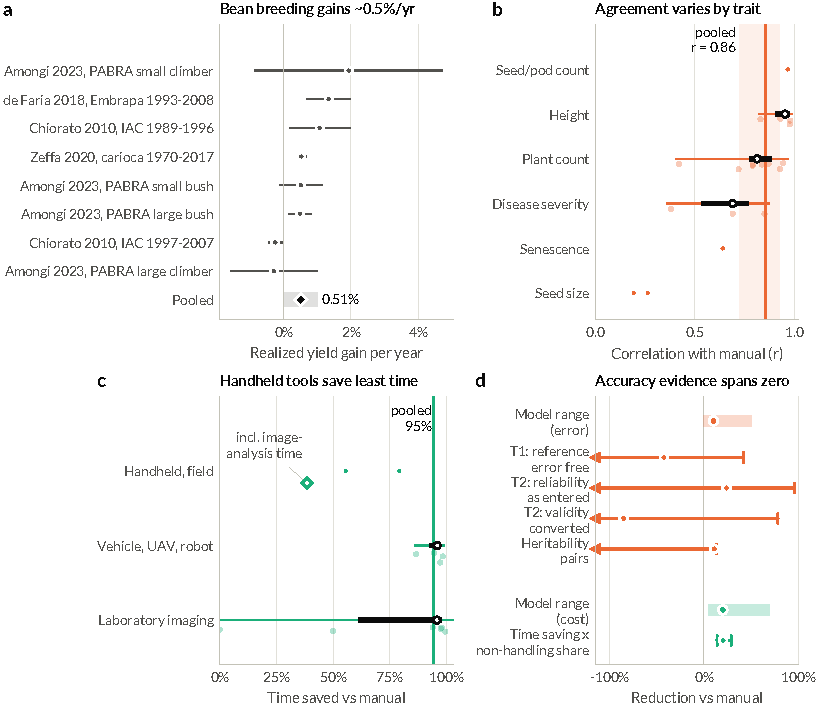
\includegraphics[width=\linewidth]{figures/fig6_evidence.pdf}
\caption{Evidence behind the model inputs. (\textbf{a}) Realized yield gain of common-bean breeding programs by program and period (dots and lines: estimates with 95\% intervals; diamond and band: three-level REML estimate and 95\% CI of the pool). IAC and Embrapa are Brazilian programs of the source studies. (\textbf{b}) Agreement between image-based or AI tools and manual reference measurements by trait (dots: individual effects; bar and ring: interquartile range and median for traits with several effects; line: pooled estimate; band: its 95\% CI). (\textbf{c}) Time saved by digital phenotyping relative to manual recording, by platform (dots: individual units; bar and ring: interquartile range and median where there are enough units; line: pooled estimate over all platforms). For handheld tools there are two descriptive units, and the open diamond is the capture-time saving of one of them when image-analysis time is counted. (\textbf{d}) Ranges of measurement-error and whole-plot cost reduction explored by the model (bars; dots: central case) against the evidence (points: median or estimate; lines: 95\% interval, or minimum to maximum for the heritability pairs; arrows: the interval continues beyond $-$115\%).\label{fig:fig6_evidence}}
\end{figure}

Digital tools save most data-capture time, handheld field tools save the least, and the implied error and cost reductions lie at the low end of the ranges the model explores (Figure~\ref{fig:fig6_evidence}c,d). Pooled over \NumMAthreeK units, digital tools reduced time per unit of data by \NumMAthreeTime\% (95\% CI \NumMAthreeTimeCIlo to \NumMAthreeTimeCIhi), a value dominated by mechanized platforms and laboratory imaging. For handheld tools in field plots, the estimates ranged from \NumMAthreeHandheldLo to \NumMAthreeHandheldHi\% (descriptive only; \NumMAthreeHandheldK units, the upper value derived from times reported for a smartphone field workflow) \cite{Walter2019Highthroughput,Lasdun2024Participatory}. When image-analysis time is counted, the capture-time saving of the lower unit fell to \NumMAthreeWalterTotal\% \cite{Walter2019Highthroughput}. A study of smartphone grain counting found no time saving \cite{Komyshev2017Evaluation}. Multiplying the share of plot cost that is not plot handling \cite{Reynolds2019Costefficient} by the field handheld time saving implies a whole-plot cost reduction of \NumMAthreeCostRed\% (range \NumMAthreeCostRedLo\ to \NumMAthreeCostRedHi\%), which is an upper bound on the saving from data capture alone.

The tool-manual correlation does not identify error reduction, because it depends on how reliable the manual reference is. The manual-reliability evidence from three studies pooled to \NumMAtwoManualRel\ (95\% CI \NumMAtwoManualRelLo\ to \NumMAtwoManualRelHi) when every coefficient was entered as a correlation with the true value. That pool mixes correlations of raters with a digital measure of the truth, correlations between two raters, and squared correlations, and the study with the first kind alone gave \NumMAtwoManualTruthOnly. After converting each coefficient to a correlation with the true value, the pooled validity of manual scoring was \NumMAtwoManualRelV\ (95\% CI \NumMAtwoManualRelVLo\ to \NumMAtwoManualRelVHi), which exceeds, although its interval includes, the break-even value of \NumMAtwoBreakEvenRel\ at which a tool correlated \NumMAtwoR\ with manual scores would equal manual scoring. The implied error reduction had a median of \NumERtOne\% when the manual reference is treated as error free (95\% interval \NumERintTOneLo\ to \NumERintTOneHi\%), \NumERtTwo\% when it carries the pooled manual error as entered (\NumERintTTwoLo\ to \NumERintTTwoHi\%), \NumERtTwoV\% after the conversion (\NumERintTTwoVLo\ to \NumERintTTwoVHi\%), and \NumERhtwoMedian\% from heritability pairs (range \NumERintHtwoLo\ to \NumERintHtwoHi\%). The heritability pairs set the central value of the model. Route T1 and the converted route T2 give negative medians, route T2 as entered gives a positive one but rests on the pool that mixes coefficient types, and the probability of a positive error reduction was \NumERprTOnePos\%, \NumERprTTwoPos\% and \NumERprTTwoVPos\% for the three correlation-based routes. The intervals or ranges of all four routes include zero improvement.

\section{Discussion}

\subsection{Where the Value Lies and Why}

In this simulation, the economic value of a smartphone phenotyping tool depends on whether the tool shortens the breeding cycle. Cycle compression is an assumed scenario input: we found no study that measured how far a phenotyping tool shortens a breeding cycle, so every value here is conditional on an assumed compression of zero to three years. Within that range, cycle compression has a total Sobol index of \NumSobolSTCyc{} for net present value (NPV), against \NumSobolSTErrRed{} for measurement-error reduction. Learning the true compression is worth \NumEVPPIIndiffCyc{} million USD at the indifference hurdle, against \NumEVPPIIndiffErrRed{} million USD for learning the error reduction (Figure~\ref{fig:fig5_what_to_measure}). Across the explored tool profiles, error reduction and cheaper plots raise per-cycle genetic gain by \NumDGdiffPct\% on average (Figure~\ref{fig:fig3_gain_ceiling}), whereas one year of compression raises annual gain by \NumCycOneYearPct\% by construction. At the central plot-level heritability of \NumCfgHtwoYield{}, the per-cycle uplift of a profile with the evidence-based error reduction equals about \NumExchMoHtwoMidErrTen months of cycle compression, and the uplift of a profile with the largest error reduction explored equals about \NumExchMoHtwoMidErrFifty months (Figure~\ref{fig:fig2_time_beats_accuracy}b). These equivalents are computed from the total per-cycle uplift of the robustness block, which also contains the effect of cheaper plots, so they overstate the share due to accuracy alone.

The ordering follows from the breeder's equation and from the model structure, so part of the dominance is structural rather than empirical. Annual gain is per-cycle gain divided by cycle length. Error reduction enters through the square root of heritability, and replication across plots and environments already averages much of the plot error \cite{Cobb2019Enhancing}. Cheaper plots convert into more entries and environments under a fixed budget, with diminishing returns \cite{Cobb2019Enhancing,Lorenz2013Resource}. Compression, in contrast, is a pure time shift in the model. It leaves stages, trial sizes and selection decisions unchanged, so the shorter cycle carries no penalty in selection accuracy or genetic variance. In the economic layer, each program's gain from one cycle accrues over its cycle and then holds constant, with later cycles not credited, so compression enters as an earlier release, a steeper accrual and an earlier adoption path inside the \NumCfgHorizon-year horizon. The horizon-dependent Sobol index of compression shows this timing effect (Figure~\ref{fig:fig4_value_follows_time}c). It is \NumDynSTCycYearFive{} before any release, when only cost phasing differs, peaks at \NumDynSTCycPeak after the first releases of the compressed program, and falls to \NumDynSTCycFinal{} at the horizon as price, discount rate and adoption ceiling gain weight.

The robustness analyses test the structure and the prior, not the existence of compression. The ranking survived a compression of at most one year or at half-year steps, a prior with probability \NumCfgZeroMassB{} on no compression, the removal of the ramp, recurrent cycles, a longer horizon, slower adoption and other calibration targets (Table~\ref{tab:robust}). The least favorable combination still gave a total index of \NumRvSTCycConservativeZeroOne{} for compression against \NumRvSTErrConservativeZeroOne{} for error reduction. These checks show that the ranking does not depend on the width of the assumed range or on the single-cycle ramp. They do not show that a tool can remove a season from the pipeline, and a compression of a few months would make accuracy and compression comparable, as the month equivalents above indicate.

\subsection{Agreement with Earlier Evidence}

The ordering agrees with breeding-program economics. Shorter cycles raised gain per year or lowered the cost of a unit of gain in analyses and simulations of rice, maize and dry bean programs \cite{Bonnecarrere2019Economic,Chaingeni2025More,Lin2023Simulations,Seck2024Stochastic}. Those studies evaluated breeding methods such as rapid generation advance, doubled haploids, speed breeding and rapid recycling. Our result transfers their logic to a phenotyping tool and holds only if the tool shortens the cycle in a comparable way. The small accuracy effect has an empirical counterpart in maize. Image-based tassel traits had lower heritability than manual traits, yet no loss of association-mapping power was detectable \cite{Gage2018Comparing}, which suggests that a measurement with lower heritability does not always degrade genetic inference. The comparison is limited, because the image traits came mostly from one environment and the manual traits from three, so their heritabilities are not directly comparable. The only economic model of phenotyping adoption that we found is theoretical, and its authors reported scarce data on cost and on the contribution of the tool to genetic gain \cite{Awada2018Adoption}. The simulation here supplies a gain contribution, conditional on its inputs.

Two caveats from the literature bound the result. Shorter cycles deplete genetic variance and selection accuracy faster \cite{Seck2024Stochastic,Jighly2019Boosting}, and under a fixed budget more cycles per year shrink the population tested in each cycle \cite{Gorjanc2018Optimal}. The model has no recurrent or rapid-cycling scheme with a selection penalty, so these trade-offs lie outside its scope, and its compression values are best read as values before any such penalty.

\subsection{When Accuracy Matters}

The model values accuracy as an effective reduction in the error variance of the selection phenotype for a single yield trait, and a smartphone imaging tool does not measure grain yield. The evidence for error reduction concerns height, counts and disease scores, and the pathway from images to lower yield-plot error is untested. The accuracy results therefore bound the value of an effect that the tool may not have, and the conclusion that accuracy is worth little is more secure than any positive value of accuracy reported here.

Accuracy carries value in three situations: when plot-level heritability is low, for traits that manual scoring measures poorly, and in programs where the tool cannot change the cycle length. At the lowest plot-level heritability explored, the per-cycle uplift of the largest error reduction equals about \NumExchMoHtwoLowErrFifty months, close to one year of compression, whatever the on-station GxE parameter (Figures~\ref{fig:fig2_time_beats_accuracy}b and~\ref{fig:fig3_gain_ceiling}c). No source reports plot-level heritability for this pipeline, so this condition is a scenario that a program can check against its own trial data. Manual scoring also differs between raters. Trained raters typically reach high concordance with a reference, whereas inexperienced raters can fall far lower \cite{Bock2021Plant}, and rater differences can change estimated allele effects, not only noise \cite{Poland2011Beholder}. In the meta-analysis, pooled agreement between tool and manual scores was lowest for disease severity among the trait groups with several estimates (Figure~\ref{fig:fig6_evidence}b). The model has a single yield trait and cannot value accuracy for visually scored traits, so where such traits drive selection, accuracy may carry more value than we report. Finally, when compression is fixed at zero, error reduction has a total Sobol index of \NumSobolCycZeroSTErrRed{}, nearly tied with the discount rate (\NumSobolCycZeroSTDisc) and ahead of price (\NumSobolCycZeroSTPrice). The value apportioned is small, however. The mean equivalent annual value across profiles without compression is \NumConsEAAmean{} USD per hectare per year (standard deviation (SD) \NumConsEAAsd{}).

\subsection{Implications for Tool Developers}

If a tool is to add value, the simulation indicates that it must bring selection decisions forward, and developers can report the quantities that a program-level valuation needs. Time saved per plot does not equal time saved per cycle. Only savings at the stage that limits a decision shorten the cycle, for example data that arrive early enough to recycle parents once first-stage results exist \cite{Seck2024Stochastic}. Handheld field tools save less time than mechanized platforms (Figure~\ref{fig:fig6_evidence}c) and can save none until the workflow is engineered. In one field deployment the first smartphone workflow was slower than visual scoring, and image analysis took back part of the capture-time saving of a handheld wheat system \cite{Lasdun2024Participatory,Walter2019Highthroughput}. Continued phenotyping is also a precondition for rapid cycling, because simulated gain plateaued when the training data were not updated \cite{Pook2025Optimization}. Throughput and cycle length are therefore complements. Tool papers could report the stage and decision the tool serves, the days saved per decision, the whole-plot cost, the error variance against an independent reference rather than the correlation with a manual score alone, and genotype-dependent bias \cite{Zhou2021Identification}. Agreement with a manual score alone cannot support a valuation of a tool's effect on a program.

\subsection{Implications for Pilots and for the Evaluation of Tools}

If cycle compression is achievable, the simulation indicates that a pilot should first measure the compression the tool delivers and measure error reduction second, against an independent reference. The value-of-information ranking supports this order. Learning cycle compression is worth \NumEVPPIIndiffCyc{} million USD at the indifference hurdle, more than any other input, and it remains the most valuable input when an annual running cost makes the decision depend on the information (Table~\ref{tab:netvalue}). Learning the discount rate (\NumEVPPIIndiffDisc{} million USD) or the bean price (\NumEVPPIIndiffPrice{} million USD) is also valuable, but a pilot cannot learn either, so they are context for scenarios. At a hurdle of zero, EVPPI is \NumEVPPIzeroHurdleMax{} million USD for every input, so the go or no-go decision is insensitive to all uncertainty in a model that excludes the cost of the tool. A pilot also cannot observe a full cycle. It should record the dates at which each stage decision becomes possible under the manual and the tool workflows, the stages at which data are the bottleneck, and the time per plot and per decision, and it should project compression from these records. Error reduction cannot be read from a tool-manual correlation. The pooled correlation (\NumMAtwoR) translates into a negative error reduction if the manual reference is treated as error-free, and into a negative one after the manual-scoring coefficients are converted to correlations with the true value, whereas the as-entered coefficients give a positive one. Repeated manual scoring of the same plots is therefore needed to estimate manual reliability. Expected value of perfect partial information is expressed in the units of the calibrated model, and exceeding the cost of research is necessary but not sufficient for research to be worthwhile \cite{Rothery2020Value}. We did not cost a pilot.

The case suggests an evaluation chain for phenotyping tools: tool metrics (agreement, time and cost), then selection gain at the program level under a fixed budget, then gain calibrated to realized progress, then adoption-weighted value, and finally attribution and value of information.

\subsection{Limitations}

The largest limitation is that cycle compression is assumed, not observed, and it enters the model structurally through the denominator of annual gain and through the timing of release. The tool is also assumed to act on selection error, although the simulated trait is yield, which a smartphone tool does not measure, and the evidence for error reduction concerns trait-level measurement error and not yield-plot error. The valuation also treats compression as free of penalty: it leaves selection decisions unchanged, credits one cycle's gain per program and contains no recurrent or rapid-cycling scheme with a selection penalty. These features favor the shorter cycle, and the shallow downside in Figure~\ref{fig:fig4_value_follows_time}d partly follows from them: both programs spend the same budget, tool costs displace plots instead of adding spending, and in the lookup table negative NPV occurs only at zero compression and only where the simulated per-cycle difference is negative. The robustness analyses vary the ramp, the horizon, the adoption rate and the prior on compression (Table~\ref{tab:robust}), and they do not remove the dependence on the assumed compression. The NPV also ignores the cost of developing, hosting and supporting the tool. The scenarios with an annual running cost (Table~\ref{tab:netvalue}) use illustrative levels that bracket a regional share of the order of magnitude reported for a global system, and a program-specific cost estimate is missing.

Second, the model treats error as random plot error that replication averages out. Image error can be genotype-dependent bias that replication does not remove \cite{Zhou2021Identification}, and a single additive yield trait omits multi-trait selection. Third, the simulation covers one cycle with fixed pipeline sizes. The cycle length is an assumption and the model's $L$ is the time from cross to release, whereas the era-trial rates used for calibration reflect many overlapping cycles. Genotype-by-environment interaction enters only through genotype-mean heritability with the parameterization of Equation~(\ref{eq:heff}), and plot-level heritability and the on-station GxE parameter are assumptions explored in the robustness block (Table~\ref{tab:inputs}).

Fourth, calibration uses one common factor (\NumGainScale{}) to match a realized gain of \NumGainTargetPct\% per year estimated from \NumMAoneKclus programs, three of them Brazilian, and the confidence interval of that estimate extends to approximately zero. Regression-based realized gain is itself imprecise \cite{Rutkoski2019Estimation}. The calibration target changes the scale of every monetary value (Table~\ref{tab:robust}). The factor is equivalent to a lower additive genetic standard deviation and keeps the relative uplift of accuracy, whereas a program that gains slowly because of low effective heritability would raise the value of accuracy. The robustness block does not reach such low heritability, because its manual gain stays far above the realized rate. Fifth, the adoption rate and midpoint are fixed assumptions in the main analysis, and the assumed rate implies faster area gain than the roughly one percentage point per year observed for improved beans \cite{Alene2019Measuring}. The simulated program is a regional network whose budget corresponds to about \NumNetProgMin{} to \NumNetProgMax{} national programs at reported maize and rice pipeline costs \cite{Das2025Costing,Katiyar2026Unified}, and its benefits are summed over the same six countries; this scope is an assumption, and a single national program would have a smaller budget and a smaller area. The model has no price or surplus effects and no farmer-level costs. NPV uses calibrated cell means, so Monte Carlo variation within a profile does not enter its distribution. Ex ante valuations tend toward optimism \cite{Hurley2014Reexamining,Flyvbjerg2021Costbenefit}, so the monetary values rank inputs and are not forecasts.

Sixth, the sensitivity analyses are exact for the grid prior, which weights every simulated level equally and is therefore a choice, not a measured distribution of the inputs. Shapley effects with correlated inputs depend on assumed correlations and no longer lie between the first-order and total Sobol indices \cite{Iooss2019Shapley}, PAWN magnitudes depend on its summary statistic \cite{Puy2020Sensitivity}, and the active-subspace check uses a piecewise constant lookup. We therefore compare ranks, not magnitudes, across measures. The four minor technical inputs cannot be ranked, because their indices are below the noise that Layer 1 simulation adds. Seventh, the meta-analyses rest on few studies with high heterogeneity, include preprints in the agreement analysis, report no variances for time savings, pool agreement across traits and platforms, and had incomplete search coverage, so ``not found'' means not found in our searches. The conversion of manual-reliability coefficients assumes parallel raters with independent errors, and the central error reduction comes from the heritability pairs, because route T1 and the converted route T2 give negative medians and route T2 as entered rests on a pool that mixes coefficient types.

\section{Conclusions}

Under an assumed cycle compression of zero to three years, which no study has measured, the simulated economic value of a smartphone phenotyping tool in a common-bean program lies in shortening the breeding cycle and not in measuring more accurately or more cheaply. Cycle compression has a total Sobol index of \NumSobolSTCyc{} for NPV, against \NumSobolSTErrRed{} for error reduction, and it kept the first rank in all \NumRvNscenarios{} robustness scenarios. At the baseline economic state, the median equivalent annual value is \NumEAAcycOne{} USD per hectare per year with one year of compression and \NumEAAcycZero{} USD without it. Learning the achievable compression is worth \NumEVPPIIndiffCyc{} million USD at the indifference hurdle, against \NumEVPPIIndiffErrRed{} million USD for learning the error reduction. These results are conditional on the assumed compression, on error reduction acting on the selection phenotype and not on measured yield, and on a valuation that excludes the cost of the tool. Accuracy mattered in the simulation only at low plot-level heritability, and the model does not address traits that manual scoring measures poorly.

If these conditions hold, the first measurement for a pilot is the cycle compression the tool achieves, and the evaluation chain from tool metrics to selection gain, adoption-weighted value and value of information gives programs and funders a basis beyond agreement with manual scores.


%=================================================================
% Back matter
\authorcontributions{Conceptualization, J.-S.T.; methodology, J.-S.T.; software, J.-S.T.; validation, J.-S.T.; formal analysis, J.-S.T.; investigation, J.-S.T.; data curation, J.-S.T.; writing---original draft preparation, J.-S.T.; writing---review and editing, J.-S.T. and J.C.; visualization, J.-S.T.; supervision, J.C.; project administration, J.C.; funding acquisition, J.C. All authors have read and agreed to the published version of the manuscript.}

\funding{This research was funded by the Beijing Academy of Agriculture and Forestry Sciences Innovation Capacity Project: Rural Revitalization Research Center (KJCX20240404) and the Beijing Academy of Agriculture and Forestry Sciences Reform and Development Program ``Agricultural Data Science Technology Research and Application'' (GGFZSJS2026).}

\institutionalreview{Not applicable.}

\informedconsent{Not applicable.}

\supplementary{The following supporting information can be downloaded at the website of this paper: Table S1: Search queries, sources and hit counts for the three meta-analyses; Figure S1: PRISMA 2020-style flow diagrams for the three meta-analyses.}

\dataavailability{The code, the Layer 1 per-replicate results and cell summaries, the Layer 2 outputs, the meta-analysis extraction sheets and the scripts that generate every number, table and figure in this article are openly available on GitHub at \url{https://github.com/juksentang/bean-phenotyping-value} and archived on Zenodo at \url{https://doi.org/10.5281/zenodo.23197205}.}

\acknowledgments{This research was enabled in part by support provided by Calcul Qu\'ebec (\url{https://www.calculquebec.ca}) and the Digital Research Alliance of Canada (\url{https://alliancecan.ca}).}

\conflictsofinterest{The authors declare no conflicts of interest.}

\abbreviations{Abbreviations}{
The following abbreviations are used in this manuscript:

\noindent
\begin{tabular}{@{}ll}
AI & artificial intelligence\\
AYT & advanced yield trial\\
CI & confidence interval\\
EAV & equivalent annual value\\
EVPPI & expected value of perfect partial information\\
GxE & genotype-by-environment interaction\\
NPT & national performance trial\\
NPV & net present value\\
ON & observation nursery\\
PABRA & Pan-Africa Bean Research Alliance\\
PI & prediction interval\\
PYT & preliminary yield trial\\
QTL & quantitative trait loci\\
REML & restricted maximum likelihood\\
RGB & red, green, blue\\
SD & standard deviation\\
UAV & unmanned aerial vehicle\\
\end{tabular}%
}

%=================================================================
\appendixtitles{yes}
\appendixstart
\appendix
\section{Appraisal of the Studies in the Tool-Manual Agreement Analysis}
\label{app:appraisal}

Table~\ref{tab:ma2appraisal} lists the effects pooled in MA2 with the quantities that bear on how much weight a single pooled correlation can carry.

\begin{table}[H]
\caption{Appraisal of the effects pooled in MA2: crop, trait, platform, type of manual reference, unit of observation (which defines $n$ in the Fisher $z$ variance $1/(n-3)$) and preprint status.\label{tab:ma2appraisal}}
\begin{adjustwidth}{-\extralength}{0cm}
\footnotesize
\setlength{\tabcolsep}{3pt}
\begin{tabularx}{\fulllength}{>{\raggedright\arraybackslash}p{1.8cm}>{\raggedright\arraybackslash}p{1.8cm}>{\raggedright\arraybackslash}p{2.2cm}>{\raggedright\arraybackslash}p{2.2cm}>{\raggedright\arraybackslash}p{2.6cm}>{\raggedright\arraybackslash}p{1.6cm}>{\raggedright\arraybackslash}X>{\raggedright\arraybackslash}p{0.8cm}>{\raggedright\arraybackslash}p{1.2cm}}
\toprule
\textbf{Study} & \textbf{Crop} & \textbf{Trait} & \textbf{Platform} & \textbf{Manual reference} & \textbf{Unit} & \textbf{Correlation entered} & \textbf{\emph{n}} & \textbf{Preprint}\\
\midrule
\cite{Volpato2023Digital} & dry bean & plant count & UAV camera & manual count & plot & 0.79 (Pearson) & 132 & yes\\
\cite{Mohammadi2024Enhancing} & faba bean & height & UAV camera & instrument measurement & plot & 0.93 (Pearson) & 152 & no\\
\cite{Guo2025Dlmlpc} & soybean & seed/pod count & smartphone & manual count & plant & 0.97 (Pearson) & 50 & no\\
\cite{McDonald2022Automated} & soybean & disease severity & camera or scanner & visual score & plant & 0.85 (Spearman $\rho$) & 2096 & no\\
\cite{Liu2021Pocketmaize} & maize & height & smartphone & instrument measurement & plant & 0.98 ($\sqrt{R^2}$) & 90 & no\\
\cite{Zang2023Fieldmeasured} & wheat & height & UAV camera & instrument measurement & plot-stage & 0.83 (Pearson) & 1920 & no\\
\cite{Zang2022Estimation} & winter wheat & height & UAV camera & instrument measurement & plot-stage & 0.98 ($\sqrt{R^2}$) & 2004 & yes\\
\cite{Banerjee2021Machine} & wheat & plant count & UAV camera & manual count & row-plot & 0.93 ($\sqrt{R^2}$) & 80 & no\\
\cite{FernandezGallego2018Wheat} & durum wheat & plant count & camera or scanner & manual count & image & 0.79 (Pearson) & 72 & no\\
\cite{FernandezGallego2018Wheat} & durum wheat & plant count & camera or scanner & manual count & image & 0.72 (Pearson) & 24 & no\\
\cite{FernandezGallego2018Wheat} & durum wheat & plant count & camera or scanner & manual count & image & 0.87 (Pearson) & 24 & no\\
\cite{FernandezGallego2018Wheat} & durum wheat & plant count & camera or scanner & manual count & image & 0.42 (Pearson) & 24 & no\\
\cite{SadeghiTehran2019Deepcount} & wheat & plant count & camera or scanner & manual count & plot & 0.94 ($\sqrt{R^2}$) & 54 & no\\
\cite{SadeghiTehran2019Deepcount} & wheat & plant count & camera or scanner & manual count & plot & 0.84 ($\sqrt{R^2}$) & 72 & no\\
\cite{Karisto2017Ranking} & winter wheat & disease severity & camera or scanner & visual score & cultivar & 0.38 (Spearman $\rho$) & 335 & yes\\
\cite{Parrella2013Evaluation} & common bean & disease severity & camera or scanner & visual score & line / plot & 0.69 (Pearson) & 12 & no\\
\cite{Gijare2026Assessing} & soybean & seed size & smartphone & instrument measurement & accession & 0.26 ($\sqrt{R^2}$) & 192 & yes\\
\cite{Gijare2026Assessing} & soybean & seed size & smartphone & instrument measurement & accession & 0.19 ($\sqrt{R^2}$) & 192 & yes\\
\cite{Makanza2018Highthroughput} & maize & senescence & UAV camera & visual score & plot & 0.64 (Pearson) & 150 & no\\
\bottomrule
\end{tabularx}
\end{adjustwidth}
\noindent{\footnotesize{Manual-reference types were coded from the description of the reference in each source. The first column gives the study, and the unit column gives what $n$ counts (plots, plants, images, accessions, lines or cultivars), so $n$ is not the number of independent genotypes. Correlations are entered as reported, with square roots of $R^2$ and Spearman coefficients treated as correlations.}}
\end{table}



%=================================================================
\begin{adjustwidth}{-\extralength}{0cm}

\reftitle{References}

\bibliography{lit/refs}

\PublishersNote{}
\end{adjustwidth}
\end{document}
